\chapter[The Higgs boson]{The Standard Model of particle physics and the Higgs boson}

Back in the 1960's the understanding of particle physics and its underlying mathematical structure was the following: fundamental particles were described as excitations of their peculiar fields, a description derived from quantum mechanics, and their interaction was governed by a lagrangian mixing those fields. In this scheme each fundamental force is associated to a field and its relative particle(s), which have integer spin value (gauge bosons). Conserved physical observables in this framework (particle's quantum numbers) are preserved by dedicated gauge symmetries introduced in the lagrangian. At that time, though, the behavior of the weak force, responsible of $\beta$ decays and more generally of all the decays with long lifetime observed in nature (e.g. the decay of the muon), could not fit in this description. Due to its long lifetime and short interaction distance, the weak force mediator was ought to be massive and the naive introduction of a mass term for a bosonic field would lead to a disruption of the gauge symmetrical properties of the lagrangian. In this period the work of several physicists, in particular of Peter Higgs and Francois Englert, led to a different formulation of the origin of mass for gauge bosons, compliant with the restrictions of a gauge-invariant lagrangian. This breakthrough led to consolidation of the model at the price of the addition of a new, theoretical, fundamental particle: the Higgs boson.

In the former part of this chapter the mathematical formulation of the current understanding of the fundamental particles and interactions, the \emph{Standard Model of particle physics} (SM), will be reviewed. In the latter part a wide review of the status of experimental searches for the Higgs boson will be presented.

\section{The Standard Model}
\subsection{Elementary particles}

Elementary particles composing ordinary and exotic matter are all \emph{fermions}, i.e. particles with spin 1/2 which obey the Fermi-Dirac statistics. These particles can be divided into two categories according to their interaction with the strong force (described later): leptons and quarks. The former are neutral with respect to the strong force while the latter carry a charge. Quarks and leptons can be divided into three families (or generation) each. Each family contains a doublet of either quarks or leptons which carry the same charges as their homologous in the other families. The only distinctive characteristic between families is the mass of their components.

This whole set-up is additionally duplicated by the presence of anti-matter. Each anti-matter particle carries the same mass, spin and lifetime as its counter-parts, but has opposite quantum charges.

\paragraph{Leptons} comprise three charged particles, the electron ($e\-$), the muon ($\mu\-$), and the tau ($\tau\-$), all carrying the same electric charge as the electron: $Q = -e = -1.602 \times 10^{-19}$ C. Each of the charged leptons is associated to a \emph{neutrino}, a particle with neutral charge and assumed massless in the SM. The recent evidence of neutrino oscillations \cite{Agafonova:2010dc} proved that neutrinos do carry a mass, albeit extremely small and not yet measured so far. 

The existence of a fourth lepton family with a light--mass neutrino associated to has been excluded by the fit of the $\Z\To$invisible production at LEP \cite{ALEPH:2005ab}. 

\paragraph{Quarks} are particles carrying fractional electric charge with respect to the charge of the electron. They carry an additional charge called \emph{colour} which allows them to interact with the strong force. The peculiar behaviour of the strong force \emph{confines} the quarks within aggregates of multiple constituents called \emph{hadrons}, making impossible the observation of ``bare'' (or ``naked'') quarks. Quarks and anti-quarks cluster in groups of two or three particles forming \emph{mesons} and \emph{baryons}, respectively. The existence of aggregates of four (anti-)quarks, called \emph{tetraquarks}, has been long postulated and only recently confirmed by the BELLE \cite{Choi:2007wga} and LHCb collaborations \cite{Aaij:2014jqa}.

Each quark family is composed by a quark with charge +2/3 and one of charge -1/3 also named ``up--type'' and ``down--type'' from the name of the constituents of the first family (which form protons and neutrons).

The presence of a fourth generation of leptons and quarks has not been completely excluded and is object of dedicated searches which review is beyond the scope of this work.

Table \ref{tab:quark_leptons} summarises the properties of quarks and leptons currently known.

\begin{table}
\caption{Fundamental particles of the SM, listed with their main properties and classification.}
\label{tab:quark_leptons}
\resizebox{0.9\textwidth}{!}{\begin{minipage}{\textwidth}
\begin{center}
\begin{tabular}{ c|c|c c c c}
\hline
 & Generation & Name & Symbol & Charge [$e$] & Mass [MeV] \\
\hline
\multirow{6}{*}{leptons} & \multirow{2}{*}{1} &  electron & $e$ & -1 & 0.511 \\
  &  &  electronic neutrino & $\nu_e$ & 0 & $< 2 \times 10^{-6}$ \\
\cline{2-6}
  & \multirow{2}{*}{2} &  muon & $\mu$ & -1 & 105.7 \\
  &  &  muonic neutrino & $\nu_\mu$ & 0 & $< 0.19$ \\
\cline{2-6}
  & \multirow{2}{*}{3} &  tau & $\tau$ & -1 & $1.78 \times 10^3$ \\
  &  &  tauonic neutrino & $\nu_\tau$ & 0 & $< 18.2$ \\
\hline
\multirow{6}{*}{quarks} & \multirow{2}{*}{1} &  up & $u$ & $+2/3$ & $2.3^{+0.7}_{-0.5}$ \\
  &  &  down & $\nu_e$ & $-1/3$ & $4.8^{+0.5}_{-0.3}$ \\
\cline{2-6}
  & \multirow{2}{*}{2} &  charm & $c$ & $+2/3$ & $(1.275\pm0.025) \times 10^3$ \\
  &  &  strange & $s$ & $-1/3$ & $95\pm5$ \\
\cline{2-6}
  & \multirow{2}{*}{3} &  top & $t$ & $+2/3$ & $(173.07 \pm0.52 \pm0.72) \times 10^3$ \\
  &  &  bottom/beauty & $b$ & $-1/3$ & $(4.18 \pm0.03) \times 10^3$ \\
\hline
\end{tabular}
\end{center}
\end{minipage}
}
\end{table}


\subsection{Elementary forces}

Elementary forces are mediated by bosons, particles with integer spin. The forces considered fundamental in the SM are:

\paragraph{The \emph{strong} interaction} is responsible of confining the quarks within the hadrons, traces of this force keep atomic nuclei stable forming a bond similar to the Van der Waals forces occurring between the molecules. The charge linked to the strong interaction is called \emph{colour}, as it can be defined in a three dimensional space. Unitary charges for the strong interaction are therefore named according to the three primary colours, red, green, and blue. Anti-colours can be defined as negative values of the fundamental colour charges. The strong interaction is mediated by eight electrically neutral and masses bosons called \emph{gluons}, each carrying a pair of color and anti-colour charges. The fundamental characteristic of the strong interaction, that differentiates it from the other fundamental forces, is that increases its strength increasing the distance between the interacting particles, leading to the confinement of the quarks. A hadron, globally neutral with respect to strong interaction, it is often referred as ``white'' due to optical color analogy.

\paragraph{The \emph{electromagnetic} interaction} is responsible for the interaction between electrically charged particles, and is empirically known to have an infinite range. The part of the SM that describes this interaction is called \emph{Quantum ElectroDynamics} (QED) and considers the interaction to be mediated by massless neutral particles called \emph{photons}, which are the EM wave quanta.

\paragraph{The \emph{weak} interaction} is responsible for most of the nuclear the decays that can be observed in nature (except the $\alpha$ and $\gamma$ nuclear decays). Its short interaction range and relative long lifetime of unstable particles decaying weakly, such as the muon, imply the mediators to be massive. The weak interaction has also been found to allow decays forbidden by the previous two interactions, such as flavour--changing decays (i.e. between different generations) and parity--violating decays. The weak interaction is mediated by two charged bosons, $\W^\pm$, of mass $m_\W = 80.4$ GeV and a neutral boson, called $\Z\0$ of $\Z$, of mass $m_\Z = 91.2$ GeV.

\paragraph{The \emph{gravitational} interaction} is responsible of the attraction between bodies. It is supposed to be mediated by a spin 2 boson called \emph{graviton}, but no evidence has been found yet. The gravitational force is not included in the SM as its strength is so faint its effect on fundamental particles is not measurable with present--day experiments and no clear theory has yet managed to couple the quantum field theory framework with the general relativity one.

A summary of the interactions is given on Table \ref{tab:bosons}.

\begin{table}
\caption{Fundamental interactions and their main properties. (a) The range of the nuclear force, not that of the quark-quark force}
\label{tab:bosons}
%\resizebox{0.9\textwidth}{!}{\begin{minipage}{\textwidth}
\begin{center}
\begin{tabular}{ c c c c c c}
\hline
Interaction & Effective coupling & Mediator & Mass [GeV] & Range [$f$m]\\
\hline
Gravitation & $10^{-39}$ & graviton & 0 & $\inf$ \\
Electromagnetism & $1/137$ & photon & 0 & $\inf$ \\
Weak force & $10^{-5}$ & $\W^\pm,\Z$ & $80.4,\,91.2$ & $10^{-3}$ \\
Strong force & $10^{-39}$ & gluon & 0 & $<1^{(*)}$ \\
\hline
\end{tabular}
\end{center}
\end{table}

\subsection{A gauge theory}

As briefly outlined in the chapter introduction, the interaction between fundamental particles is described with the langrangian formalism. The sum of the charges under a specific interaction carried by each fundamental particle in the system is therefore seen as a conserved quantity. In order to protect this quantity a dedicated symmetry is introduced in the form of a local \emph{gauge symmetry}. 

In analogy with the lagrangian formalism in classical mechanics, the conserved quantity is seen as the generator of this peculiar symmetry of the system. A Noether current is also associated to each charge and symmetry of the lagrangian. The quantization of this symmetry leads to the presence of a vectorial field. 

To each gauge symmetry it is associated a lie group. Fundamental particles and force mediators are then expressed under one of the fundamental representations of such group, fully determining the behavior of the final theory.

The behavior of a free fundamental particle of spin $^1/_2$ is described by the Dirac lagrangian

\begin{equation}
\l=\psi(i\slash{\d}-m)\psi
\label{eq:dirac_lag}
\end{equation}

from which it is possible to derive the Dirac equation.

In this framework the electromagnetic interaction can be described by the U(1) lie group, whose associated symmetry is a change of phase of the spinorial field: % associated to the fundamental particles:

\begin{equation}
\psi'(x) = e^{iq\theta}\psi(x)
\end{equation}

A complex field represents here a charged particle, and the spin behavior is handled by the matrix nature of the $\psi$ field.

The behavior of a free photon, the gauge boson associated to the electromagnetic force, is described by the lagrangian

\begin{equation}
\l = -\frac{1}{4}F_{\mu\nu}F^{\mu\nu}
\end{equation}

where

\begin{equation}
 F_{\mu\nu} =\partial_{\mu}A_{\nu}-\partial_{\nu}A_{\mu}
\end{equation}

The minimal coupling between a spinorial and a photon field is described by the interaction lagrangian

\begin{equation}
\l = iq \bar{\psi} \slash{A} \psi 
\end{equation}

The full electromagnetic lagrangian can be therefore written as:

\begin{equation}
\l_{QED} = \psi(i\slash{\calD} - m)\psi - \dfrac{1}{4} F_{\mu\nu} F^{\mu\nu}
\end{equation}

Where $\slash{\mathcal{D}} = \d_\mu + i q A_\mu$ and is the extension of $\d$ to ensure the covariance of the lagrangian and additionally embeds the interaction between the fermions and the photon.

The strong interaction is described by the SU(3) group and its associated gauge symmetry, which is generated by the Gell-Mann matrices, $\tau_a$. A fundamental property of such group is that it is not \emph{abelian}, i.e. the generator matrices do not commute. The commutation rules of the SU(3) group, as any other lie group, are determined by its \emph{structure constants} $[\tau_a, \tau_b] = i C_{abc} \tau^c$. This property leads to small modification of gauge bosons lagrangian (Eq. \ref{eq:qcd_free}) and of the coupling with the quarks (Eq. \ref{eq:qcd_int}).

\begin{equation}
\l_{gluons} = - \dfrac{1}{4} G^{a}_{\mu\nu}  G_{a}^{\mu\nu}, \, \, F^{a}_{\mu\nu} = \d_\mu G^a_\nu - \d_\nu G^a_\mu -i g_s C_{abc} A^b_\mu A^c_\nu
\label{eq:qcd_free}
\end{equation}

\begin{equation}
\l_{quarks} = \bar{\psi} ( i (\slash{\d} + i g_s \slash{G}^a \tau_a) - m ) \psi = \bar{\psi} ( i \slash{\calD} - m ) \psi
\label{eq:qcd_int}
\end{equation}

The presence of trilinear and quartic terms in Eq. \ref{eq:qcd_free} describe the self--interaction between gluons, which is allowed already at the first order of perturbative expansion (also referred as \emph{tree level} or \emph{Born approximation}). The field theory describing strong interactions is called \emph{quantum chromodynamics} (QCD).

\subsection{Discrete and continuous symmetries}

In addition to the gauge symmetries described in the previous section, three discrete symmetries are of particular interest in quantum field theory: charge conjugation (C ), parity (P ), and time reversal (T). The property of these symmetries is more easily described by their effect on a quantum state $\ket{f(\vec{p}, h)}$ containing a single particle $f$ of momentum $\vec{p}$ and elicity $h = \vec{s} \cdot \vec{p} / p$, i.e. the projection of the spin along the direction of motion.

The charge conjugation operator C inverts the charge of such state transforming it in its anti-particle homologous: $C\ket{f(\vec{p}, h)} = \eta_C\ket{\anti{f}(\vec{p}, h)}$, where $\eta_C$ is a phase factor. The parity operator P inverts the spatial coordinates, it is often referred as the left-right symmetry: $P\ket{f(\vec{p}, h)} = \eta_P\ket{f(-\vec{p}, -h)}$, where $\eta_P$ the parity of the particle. The time inversion operator T inverts time leading to: $T\ket{f(\vec{p}, h)} = \eta_T\ket{f(-\vec{p}, h)}^*$, where $\eta_T$ is a phase factor depending on the spin of the particle.

Both electromagnetic and strong interaction preserve these three symmetries, while the weak force was experimentally found to violate the charge and parity conjugations. Moreover in 1964 it has been reported the first experimental evidence of CP (charge and parity combined) violation in the K meson sector \cite{PhysRevLett.13.138} due to the weak force. The weak force was found to couple only to ``left-handed'' particles, i.e. particles whose elicity is negative. More recently the same behavior has been found in B mesons decays and is still currently a lively field of study. 

Up to now no evidence of CPT violation has been experimentally observed. An hypothetical observation of CPT violation would have very strong consequences in our understanding of the underlying structure of the fundamental interaction as this symmetry forbids particles and anti-particles to have different mases or lifetime and is linked to the statistics to which fermions and bosons obey.

\section{The electroweak force}

In the description of the standard model presented so far the weak force has not been detailed yet. The nature of this interaction has been in fact extremely difficult to model in a quantum field theory framework.

The first attempt to model the weak interaction dates back to 1933 by Fermi, who suggested for the muon decay the following interaction lagrangian:

\begin{equation}
\l_{Fermi} = \sqhalf G_F \bar{\nu}_\mu \gamma_\alpha (1-\gamma^5) \mu \bar{e} \gamma^\alpha (1-\gamma^5) \nu_e
\end{equation}

Where $G_F = 1.166 \cdot 10^{-5}$ GeV$^{-2}$. This lagrangian consists of a single point-like interaction among four fermions and correctly reproduces the muon decay at tree level. Increasing the degree of the perturbative expansion, though, several divergencies arise that cannot be cancelled or renormalized, leading to a violation of unitarity and a breakdown of the theory. It has also been demonstrated that this behavior can be immediately recognised by the dimensionality of the coupling constant.

It was later shown by Glashow in 1961 \cite{Glashow:1961tr} and Salam and Ward \cite{Salam:1961en} in the same year that the weak interaction could be modeled in a quantum field theory with the SU(2) group and its related gauge bosons. 
The four-fermion interaction present in the Fermi lagrangian gets split into two interaction points connected by a charged vector boson named W$^\pm$. In order to obtain the same parity violating properties as observed in the experiments the gauge group had to be extended to SU(2)$\times$U(1), introducing a mixing between the gauge bosons. This theory showed to be reprenting not only weak interaction, but also the electromagnetic one. 
The new modeling of these fundamental interactions was finally completed by Weinberg in 1967 \cite{Weinberg:1967tq}, who named it \emph{electroweak theory}. 
As the weak interaction couples only to left-handed particles, the gauge group is sometimes noted as SU(2)$_L$, to remind this feature.

Since the generator of the fundamental representation of SU(2) are the Pauli matrices (noted as $\sigma_i$, $i \, \epsilon \, [1,3]$) it is possible to extend the spin formalism to the weak interaction. In this case the quantum number (or charge) carried by the fundamental particles is called \emph{weak isospin}, noted with I. The gauge bosons linked to the generators of the symmetry will be noted as $W^i$. Left-handed fermions are considered to carry total isospin 1/2 and are grouped in doublets of the form.

\begin{equation}
L_f = \left(\begin{array}{c}f_{up} \\f_{down}\end{array}\right)
\end{equation}

Doublets can be divided in ``up--type'' and ``down--type'' fermions, where the former are considered to have the third component of the isospin I$_3 = +1/2$, while the latter have I$_3 = -1/2$. Up--type fermions are the neutrinos and the up, charm and top quarks, while down--type fermions are the charged leptons and the down, strange, and bottom quarks.

The right--handed fermions were experimentally found to not interact weakly and therefore carry no charge. They are represented as singlets under the SU(2) group.

Left and right handed components of the fermions can be obtained by using the appropriate projector on the fermionic field: $\dfrac{1}{2}(1-\gamma^5)$ and $\dfrac{1}{2}(1+\gamma^5)$, respectively.

It is worth noting that quark flavor eigenstates under the weak interaction are not necessary also mass eigenstates, but rather a superimposition of them, giving raise to a mixing matrix. The mixing matrix has been first suggested by Cabibbo in 1963 \cite{Cabibbo:1963yz} and later by Kobayashi and Maskawa in 1973 \cite{Kobayashi:1973fv}.

The additional U(1) symmetry preserves a quantum number called \emph{hypercharge}, Y, and is connected to a gauge boson, noted with $B$. 

In this framework the derivative present in the Dirac lagrangian, shown in Eq. \ref{eq:dirac_lag}, is replaced by its covariant form:

\begin{equation}
\calD^L_\mu = \d_\mu - ig\dfrac{\sigma_i}{2}W^i_\mu - ig'\dfrac{Y}{2}B_\mu
\end{equation}

Since the transformations under SU(2) and U(1) are independent, two coupling constants, $g$ and $g'$, are assigned. The lagrangian therefore becomes

\begin{equation}
\l = \sum^f i \bar{L_f}\slash{\calD}^LL_f + \bar{f^{up}_R}\slash{\calD}^Rf^{up}_R  + \bar{f^{down}_R}\slash{\calD}^Rf^{down}_R 
\end{equation}

Where $f^{up}_R$ and $f^{down}_R$ are the right handed up and down fermions fields, respectively. Since they are singlets under SU(2) they are presented separately, but they still transform under U(1). To account for this effect we have defined $\calD^R$, which is the same as $\calD^L$, but lacks the couplings with the $W$ fields. 

We can now restrict ourselves to the electron family, without losing any generality, and identify in the lagrangian a charged and a neutral current:

\begin{eqnarray}
\l_{charged} &=& g \bar{L} \slash{W}_1 \dfrac{\sigma_1}{2}L + g \bar{L} \slash{W}_2 \dfrac{\sigma_2}{2}L \\ 
\l_{neutral} &=& \dfrac{g}{2} W_3^\mu (\bar{\nu}_{e,L}\gamma_\mu\nu_{e,L} - \bar{e}_L\gamma_\mu e_L) +  \nonumber \\
& & + \dfrac{g'}{2} B^\mu ( Y(L) ( \bar{\nu}_{e,L}\gamma_\mu\nu_{e,L} + \bar{e}_L\gamma_\mu e_L ) + \nonumber \\
& & + Y(\nu_R) \bar{\nu}_{e,R}\gamma_\mu\nu_{e,R} + Y(\nu_R)  \bar{e}_R\gamma_\mu e_R )
\end{eqnarray}

The charged part of the lagrangian contains off-diagonal Pauli matrices that mix the neutrino and electron fields. Operating the substitution:

\begin{equation}
W^\pm_\mu = \frac{1}{\sqrt{2}}(W^{1}_{\mu} \mp i W^{2}_{\mu})
\label{eq:wpm_def}
\end{equation}

it is possible to rewrite the charged part of the lagrangian as:

\begin{equation}
\l_c = \frac{g}{\sqrt{2}}(\bar{L}\slash{W}^{+} \sigma^{+} L +\bar{L}\slash{W}^{-}\sigma^{-} L)
\end{equation}

where:

\begin{equation}
\sigma^+ = \spinmatrix{0}{1}{0}{0}\,\, \sigma^- = \spinmatrix{0}{0}{1}{0}
\end{equation}

In the neutral part of the lagrangian neither $W^3$, nor $B$ can be directly identified with the photon since they both interact with the neutrino, which has no electric charge. The two gauge bosons have the same quantum numbers ($Q = 0$ and $J^P = 1^-$), it is therefore possible to create a linear combination of the two fields which represent the electromagnetic photon.

\begin{equation}
\left\{\begin{matrix}
B^{\mu}=A^{\mu}\operatorname{cos}\theta_{W}-Z^{\mu}\operatorname{sin}\theta_{W}\\ 

W^{\mu}_3=A^{\mu}\operatorname{sin}\theta_{W}+Z^{\mu}\operatorname{sin}\theta_{W}\\ 
\end{matrix}\right.
\label{eq:su2_rotation}
\end{equation}

This linear combination can be seen as a rotation of the fields by a $\theta_W$ angle, called \emph{Weinberg angle}. 
The neutral part of the lagrangian therefore becomes:
 
\begin{equation}
\l_{N}=\bar{\Psi}\gamma_{\mu}(g\operatorname{sin}\theta_{W}T_3+ \frac{Y}{2}g'\operatorname{cos}\theta_{W})\Psi A^{\mu}+\bar{\Psi}\gamma_{\mu}(g\operatorname{cos}\theta_{W}T_3- \frac{Y}{2}g'\operatorname{sin}\theta_{W})\Psi Z^{\mu}
\end{equation}

where:

\begin{equation}
\Psi = \begin{pmatrix}
\nu_L\\ 
e_L\\ 
\nu_R\\ 
e_R
\end{pmatrix}, \, \, \, T_3 = {\rm diag}\left(\frac{1}{2},-\frac{1}{2},0,0\right)
\end{equation}

In this lagrangian the boson $A$ can be identified with the QED photon. Similarly to what happens to the fields, the electric charge can be written as a linear combination of the third component of the weak isospin and the hypercharge. The charge operator can be derived from the coupling of the photon field to the fermions obtaining: 

\begin{equation}
Q = T_3 + \dfrac{Y}{2}
\end{equation}

Which, in the case of the electron family leads to the relations:

\begin{equation}
g \opname{sin}\theta_W = g' \opname{cos}\theta_W = e
\end{equation}

Which links the coupling constants and the electron charge to the value of $\theta_W$. The sine and cosine of the Weinberg angle can be therefore defined as:

\begin{equation}
\left\{\begin{matrix}
\operatorname{sin}\theta_W = \dfrac{e}{g} = \dfrac{g'}{\sqrt{g^2+g'^2}}\\ 
\operatorname{cos}\theta_W = \dfrac{e}{g'} = \dfrac{g}{\sqrt{g^2+g'^2}}
\end{matrix}\right.
\label{eq:win_angle}
\end{equation}

The identification of the $A$ boson with the photon completely determines the choice of the quantum numbers of the fundamental particles also defining their coupling to the new bosonic $Z$ field. At the time of the formulation of the electroweak theory the presence of this new boson, the Z, was yet to be observed.

The interaction between the gauge boson fields is described by the following lagrangian:

\begin{equation}
\l_g = -\dfrac{1}{4}W^a_{\mu\nu}W_a^{\mu\nu} -\dfrac{1}{4}B_{\mu\nu}B^{\mu\nu}
\label{eq:weak_free}
\end{equation}

Where in this case $W$ and $B$ represent the \emph{field strength tensor} for the relative field. As in the QCD formalism, the SU(2) generators do not commute with each other creating additional trilinear and quartic terms in the lagrangian that allow for interactions between the gauge fields.

The short range experimentally observed in the weak interaction necessitates the presence of massive gauge bosons. The naive introduction of a mass term in the lagrangian in the form

\begin{equation}
\l = -\frac{1}{16\pi}F^{\mu\nu}F_{\mu\nu}+\frac{1}{8\pi}m^2 A^{\nu}A_{\nu}
\label{eq:weak_free}
\end{equation}

leads to a violation of the gauge invariance, which allows the theory to be perturbative and renormalizable.

\section{The Higgs mechanism}

\subsection{Spontaneous symmetry breaking}

Let us consider now a field theory comprising N scalar massless fields $\vec{\phi(x)} = (\phi_1(x),\ldots,\phi_N(x))$, and a lagrangian of the form:

\begin{equation}
\l_\sigma = \half \d_\mu \vec{\phi(x)} \d^\mu \vec{\phi(x)} - V(|\vec{\phi(x)}|)
\label{eq:lin_sigma}
\end{equation}

The lagrangian shows a global invariance O(N) under the field rotations $\phi'_i(x) = R_i^j \phi_j(x)$. 

If we now choose a potential of the type:

\begin{equation}
V(|\vec{\phi(x)}|) = - \half \mu^2 |\vec{\phi(x)}|^2 + \dfrac{\lambda}{4} (|\vec{\phi(x)}|^2)^2
\label{eq:lin_sigma}
\end{equation} 

with both $\lambda$ and $\mu > 0$. It must be noted that with $\mu > 0$ the quadratic term has the wrong sign to be considered a mass for the field, and therefore the potential interpretation is consistent.

The perturbative expansion of the theory has to be performed around the classical vacuum configuration, which is the minimum of the potential. In this case the minimum is independent from the field configuration and is $|\vec{\phi(x)}|^2 = \mu^2 / \lambda \neq 0$, which is degenerate and symmetric with respect to O(N).

We can arbitrarily choose a vacuum configuration and parametrize the fields accordingly

\begin{equation}
\phi_0^i = (0, \ldots, v), \, v= \dfrac{\mu}{\sqrt{\lambda}}, \, \phi^i(x) = (\pi^k(x), v + \sigma(x))
\end{equation}

Where the index $k$ runs over $N-1$ indices. 

Substituting the new fields into the lagrangian it is possible to obtain several components:

\begin{eqnarray}
\l_{kin} &=& \half \d_\mu \pi^k \d^\mu \pi_k + \half  \d_\mu \sigma \d^\mu \sigma \nonumber \\
\l_{\sigma \, mass} &=& \half \mu^2 \sigma^2 - \dfrac{6}{4} \lambda v^2 \sigma^2 = - \mu^2 \sigma^2 = -\half (2\mu^2) \sigma^2 \nonumber \\
\l_{\pi \, mass} &=& 0 \nonumber \\
\l_{int} &=& - \dfrac{\lambda}{4} (\pi^k\pi_k)^2 - \dfrac{\lambda}{4} \sigma^4 - \dfrac{\lambda}{2} \sigma^2 \pi^k \pi_k - \sqrt{\lambda} \mu \sigma \pi^k \pi_k - \sqrt{\lambda} \mu \sigma^3 \nonumber \\
\l_{vac} &=& \dfrac{\mu^4}{4\lambda} 
\end{eqnarray}

In this final lagrangian the initial O(N) symmetry is broken, as it is evident from the special meaning that the $\sigma$ boson acquires. A residual O(N-1) symmetry is still present among the $\pi^k$ fields.
We can assign to the different fragments of the lagrangian special meanings, related to couplings expressed:
\begin{itemize}
\item $\l_{kin}$ represents the kinetic term for $N$ scalar bosons, as in the beginning of our model;
\item $\l_{\sigma \, mass}$ arise after the spontaneous breaking of the O(N) symmetry and represent a mass term for the $\sigma$ boson. No mass term is assigned to the $\pi$ fields, though;
\item $\l_{int}$ contains triple and quartic couplings among the fields, in which $\sigma$ gains a special status, breaking the initial O(N) symetry;
\item $\l_{vac}$ represents the energy of the vacuum, the vacuum expectation value of the $\sigma$ boson. Classically this term can be neglected, as only energy differences are physical observables.
\end{itemize}

This example can be generalized in the \emph{Goldstone theorem} \cite{1962PhRv..127..965G}, which states that a theory containing $K$ global symmetry generators, out of which $d$ are broken by the choice of the potential and therefore of the vacuum, $K - d$ massless bosons arise, called goldstone bosons. 

In our case the inital O(N) symmetry has $N(N-1)/2$ generators of the symmetry, while the final O(N-1) one has $(N-1)(N-2)/2$, leaving a difference of $N-1$ broken generators, leading to the $\pi$ fields being massless. 

This mechanism is valid both in quantum field theory and in quantum dynamics, where it has significant impacts in the description of superconductivity.

\subsection{The Higgs mechanism}

The previously described mechanism has been studied in the context of a gauge field theory by several authors, with Higgs and Englert among them, reporting their results in 1964 \cite{Englert:1964et, Higgs:1964ia}. The combination of these studies with the SU(2)$\times$U(1) formalism led, as said, to the definition of the electroweak theory by Weinberg and Salam in 1967.

If we now take, in the framework of the electroweak theory, a complex doublet under SU(2)

\begin{equation}
\phi = \left(\begin{array}{c}\phi_1 \\\phi_2\end{array}\right)
\end{equation}

and choose a potential of the kind:

\begin{equation}
V(\phi) = - \mu^2 |\phi|^2 + \lambda (|\phi|^2)^2
\end{equation}

with both $\lambda > 0$ and $\mu > 0$, we find that the minimum of the potential occurs at 

\begin{equation}
\phi\dag\phi = \dfrac{\mu^2}{2\lambda} \equiv \dfrac{v^2}{2}
\end{equation}

We can therefore define the vacuum state as

\begin{equation}
\phi_0 = \dfrac{1}{\sqrt{2}} \left(\begin{array}{c}v_1 \\v_2\end{array}\right)
\end{equation}

where $|v_1|^2 + |v_2|^2 = v^2$.

If we now impose that the vacuum state is neutral, i.e. $Q\phi_0 = 0$, 

\begin{equation}
Q\phi_0 = \left(\begin{array}{cc}Q_1 & 0 \\0 & Q_2\end{array}\right)   \dfrac{1}{\sqrt{2}} \left(\begin{array}{c}v_1 \\v_2\end{array}\right) = \dfrac{1}{\sqrt{2}} \left(\begin{array}{cc}\half + \dfrac{Y}{2} & 0 \\0 & -\half + \dfrac{Y}{2}\end{array}\right) \left(\begin{array}{c}v_1 \\v_2\end{array}\right) = \left(\begin{array}{c}0 \\0\end{array}\right)
\end{equation}

leading to
\begin{equation}
(1+Y)v_1 = (1-Y)v_2 = 0
\end{equation}

we obtain therefore two allowed configurations:

\begin{enumerate}
\item $v_1 = 0, \, v_2 = v, \, Y = 1$
\item $v_1 = v, \, v_2 = 0, \, Y = -1$
\end{enumerate}

In the former case $\phi_1$ is positive and $\phi_2$ is neutral, while in the latter $\phi_1$ is neutral and $\phi_2$ has negative electric charge. It can be shown that the two configurations are equivalent though, as in both cases the charged scalar is made of goldstone bosons of the theory and has no physical meaning alone.

We choose as a convention the first option and we decompose the $\phi_i$ fields in their real and imaginary components:

\begin{equation}
\phi(x) = \spinor{\phi^{(+)}(x)}{\phi^{(0)}(x)} = \sqhalf \spinor{ \pi_1(x) + i \pi_2(x) }{ v + H(x) + i \pi_3(x) }
\end{equation}

where, as in the previous example, the $\pi$ fields are the goldstone bosons.  To allow a proper renormalization, these fields have to be kept in the lagrangian, but for our purposes we can set the unitary gauge conditions and obtain:

\begin{equation}
\phi(x) = \sqhalf \spinor{ 0 }{ v + H(x) }
\end{equation}

Where $H$ is the Higgs boson field.

After this transformation the potential becomes:

\begin{equation}
V(\phi) = -\dfrac{\mu^4}{4\lambda} + \mu^2H^2 + \lambda v H^3 + 2 \lambda v^2
\end{equation}

From the potential a mass term for the Higgs boson arises: $m^{2}_H = 2\mu^2 = 2 \lambda v^2$. There are additional triple and quartic Higgs boson self--couplings that appear in the potential description. As said before, the additional $2 \lambda v^2 = m^{2}_H$ can be neglected when measuring physical observables. This term, though, gains importance once a coupling with gravity is introduced and can be linked to the cosmological constant $\Lambda$ of the general relativity theory.

The power of the spontaneous symmetry breaking mechanism becomes apparent when computing the interaction lagrangian for the $\phi$ field:

\begin{equation}
\l_{int} = (\calD_\mu\phi)\dag\calD^\mu\phi
\end{equation}

where

\begin{eqnarray}
\calD_\mu \phi &=& (\d_\mu - ig\dfrac{\sigma_i}{2}W^i_\mu - ig'\dfrac{Y}{2}B_\mu) \sqhalf \spinor{0}{v+H(x)} \nonumber \\
&=& \sqhalf \spinor{0}{\d_\mu H(x)} - \dfrac{i}{2\sqrt{2}} (v+H(x)) \spinor{g(W_{1\mu} - i W_{2\mu})}{-g W_{3\mu} + g'B_\mu}
\end{eqnarray}

Using the relations described in Eq. \ref{eq:win_angle}, \ref{eq:su2_rotation}, and \ref{eq:wpm_def} we can rewrite the spinor as function of the physical weak vector bosons:

\begin{equation}
\spinor{g(W_{1\mu} - i W_{2\mu})}{-g W_{3\mu} + g'B_\mu} = \spinor{gW^+_{\mu}}{-\sqrt{\dfrac{g^2+g'^2}{2}}Z_\mu}
\end{equation}

The interaction lagrangian then becomes:

\begin{equation}
\l_{int} = (\calD_\mu\phi)\dag\calD^\mu\phi = \frac{1}{2}\partial_{\mu}H\partial^{\mu}H+(v+H)^2\left[\frac{g^2}{4}W^+_{\mu}W^{\mu-} + \frac{1}{8}(g^2+g'^2) Z^{\mu}Z_{\mu}\right ]
\end{equation}

In which quadratic terms of the $W$ and $Z$ fields appear with the correct sign to be interpreted as a mass term. 

With the Higgs mechanism it has been possible to introduce a mass term for the gauge bosons without breaking the underlying gauge symmetry of the lagrangian. 

A common representation of this method arises from the computation of the elicity states of the gauge bosons: massless bosons have only two possible elicity states, while massive boson have an additional one. The goldstone bosons can be viewed as the additional degree of freedom that is absorbed by the weak bosons to become massive.

The mass of the weak bosons is determined by their coupling of the Higgs boson: 

\begin{equation}
M^2_W=\frac{1}{4}g^2v^2, \, \, \, \, M^2_Z=\frac{1}{4}(g^2+g'^2)v^2
\end{equation}

Additionally, the following relation between the Z and W bosons mass holds:

\begin{equation}
\frac{M_W^2}{M_Z^2}=\frac{g^2}{g^2+g'^2}=\operatorname{cos^2}\theta_W
\end{equation}

\subsection{Couplings to gauge bosons}

The interaction lagrangian contains additional terms describing the interaction of the Higgs boson with the weak gauge bosons. No direct coupling with the photon is predicted. The vertices allowed by the theory include vertices with two gauge bosons and one or two Higgs bosons. In addition, the vertices do not mix W and Z bosons. The coupling constants of these vertices are proportional to the mass of the gauge bosons interested and can be written as:

\begin{equation}
g_{HVV}=\frac{2m^2_V}{v}, \,\,\,   g_{HHVV}=\frac{2m^2_V}{v^2}
\end{equation}

Where V can be either the W or the Z boson, and $v$ is the vacuum expectation value of the Higgs boson which can be derived from the Fermi constant by the relation $v = (\sqrt{2}G_F)^{-1/2} \approx 246$ GeV.

\subsection{Couplings to fermions}

The introduction of a mass term for fermions as in the Dirac equation 

\begin{equation}
\l_{m,Dirac}= -m\bar{\psi}\psi=-m(\bar{\psi}_L\psi_R+\bar{\psi}_R\psi_L)
\end{equation}

would break the SU(2) gauge invariance of the lagrangian as it directly mixes left and right handed components of the fermionic fields, which transform differently under SU(2). To introduce the mass term for the fermions without breaking the gauge invariance it is possible to resort again on the spontaneous symmetry breaking mechanism and the $\phi$ field. A \emph{Yukawa}--type coupling
\footnote{This coupling was initially introduced by Yukawa \cite{Yukawa:1935xg} to describe the interactions between hadrons, postulating a new boson mediator, the \emph{pion}}:

\begin{equation}
\l_{Yuk}=-g_f(L_f \phi d^f_R + d^f_R \phi^{\dag} L_f)
\end{equation}

respect the gauge invariance and can produce the desired mass terms which becomes:

\begin{equation}
m_f = \frac{g_f v}{\sqrt{2}}
\end{equation}

In addition to the masses of the different fermions a term coupling the fermions with the Higgs boson appears with strength proportional to the fermion mass:

\begin{equation}
g_{Hff}=i\frac{m_f}{v}
\end{equation}

This procedure assign mass to the down--type fermions. To achieve the same results for the up--type ones it is possible to consider the coupling of the Higgs charge conjugate

\begin{equation}
\phi_C = i \sigma_2 \phi^{\ast} = \frac{1}{\sqrt{2}}=\begin{pmatrix}
v+H\\ 
0
\end{pmatrix}
\end{equation}

obtaining equivalent results for the up--type sector.

As anticipated in the previous sections, mass eigenstates do not correspond to weak ones. To model this effect it is possible to introduce a mixing matrix, the \emph{CKM} matrix, in the equations. 

\section{The Higgs boson at LHC}

\subsection{Higgs production}

The Large Hadron Collider (LHC) is the most advanced accelerator present at CERN, Geneva, where two proton beams collide with a center--of--mass energy $\sqrt{s} = 8$ TeV. A more detailed description of the accelerator and the experimental set--up is available in the following chapter.

Protons are not fundamental ``point--like'' particles, but are made by three valence quarks: two up quarks and a down one. In addition to these valence quarks, the quantum vacuum and the binding energy among the quarks produces around them a cloud of virtual quarks and gluons that can also be accessed during a collision process. The exact constitution of the proton is impossible to compute from theoretical assumptions as the QCD is not perturbative at that energy scale. The momentum carried by each constituent, valence or virtual, is also a continuous function that has to be probed experimentally. 

The probability for a quark or a gluon to be observed within a proton, with a certain momentum $p = x \cdot p_{proton}$, with $x \, \epsilon \, [0,1]$, is encoded in the parton distribution functions, measured experimentally. Figure \ref{fig:pdf} shows an example of a parton distribution function for the proton.

\begin{figure}
\centering
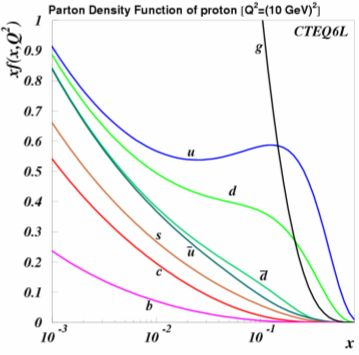
\includegraphics[width=0.5\textwidth]{1_Introduction_Th_and_Exp/pics/pdf.jpg}
\caption{Parton distribution function of the proton.}
\label{fig:pdf}
\end{figure}

As it is evident from the previous picture, the overwhelming majority of the partons present in the protons are gluons, especially at low $x$. This effects directly translate in a dominance of the gluon--fusion process in the Higgs boson production at the LHC. The Feynman diagram sketching the gluon fusion process is shown in Figure \ref{fig:ggf}. The loop inside the gluon fusion process is dominated in the SM by the top quark, since it has the largest mass in the standard model, but may receive additional contribution from new physics. 

The second largest contribution to the total Higgs production cross section comes from the vector boson fusion process (Figure \ref{fig:vbf}) in which two quarks radiate two weak bosons that then fuse producing a Higgs boson. The scattered quarks produce two high transverse momentum (\pT) jets in the forward/backward direction that can be used to experimentally tag the events.

The third most significant production mode is the so called \emph{Higgsstralhung}, or associated production with a vector boson (Figure \ref{fig:vh}). This work is focused on this production mechanism. Even though the production cross section is significantly lower than the previous two processes, the presence of a vector boson reduces greatly the background contamination. This process is also the leading source of Higgs bosons at lepton colliders.

Finally, the least Higgs production process is $tt$H, the production in association with top quarks (Figure \ref{fig:tth}). 

The production cross sections of the single processes depend both on the mass of the Higgs boson, a free parameter of the SM, and on the center--of--mass energy of the two colliding beams. Figure \ref{fig:hxs} shows the production cross section as function of the Higgs mass at 7 and 8 TeV.

\begin{figure}
        \centering
        \begin{subfigure}[b]{0.3\textwidth}
                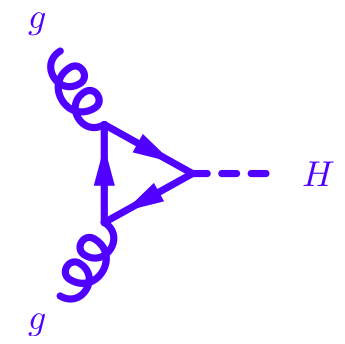
\includegraphics[width=\textwidth]{1_Introduction_Th_and_Exp/pics/ggFusion.png}
                \caption{Gluon fusion}
                \label{fig:ggf}
        \end{subfigure}%
        ~ 
        \begin{subfigure}[b]{0.3\textwidth}
                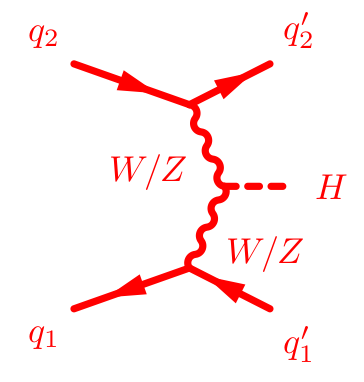
\includegraphics[width=\textwidth]{1_Introduction_Th_and_Exp/pics/BosonFusion.png}
                \caption{Vector boson fusion}
                \label{fig:vbf}
        \end{subfigure}

        \begin{subfigure}[b]{0.3\textwidth}
                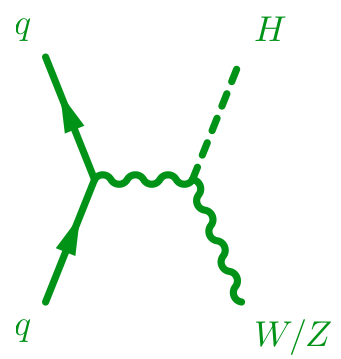
\includegraphics[width=\textwidth]{1_Introduction_Th_and_Exp/pics/Higgsstralhung.png}
                \caption{Higgsstralhung or associated production}
                \label{fig:vh}
        \end{subfigure}
        ~ 
        \begin{subfigure}[b]{0.3\textwidth}
                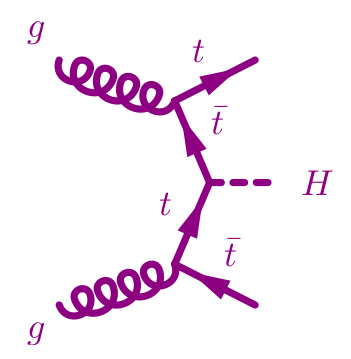
\includegraphics[width=\textwidth]{1_Introduction_Th_and_Exp/pics/ttFusion.png}
                \caption{$tt$H}
                \label{fig:tth}
        \end{subfigure}
        \caption{Tree--level Feynman diagrams for the main Higgs boson production mechanism at LHC}\label{fig:hprod}
\end{figure}

\begin{figure}
        \centering
	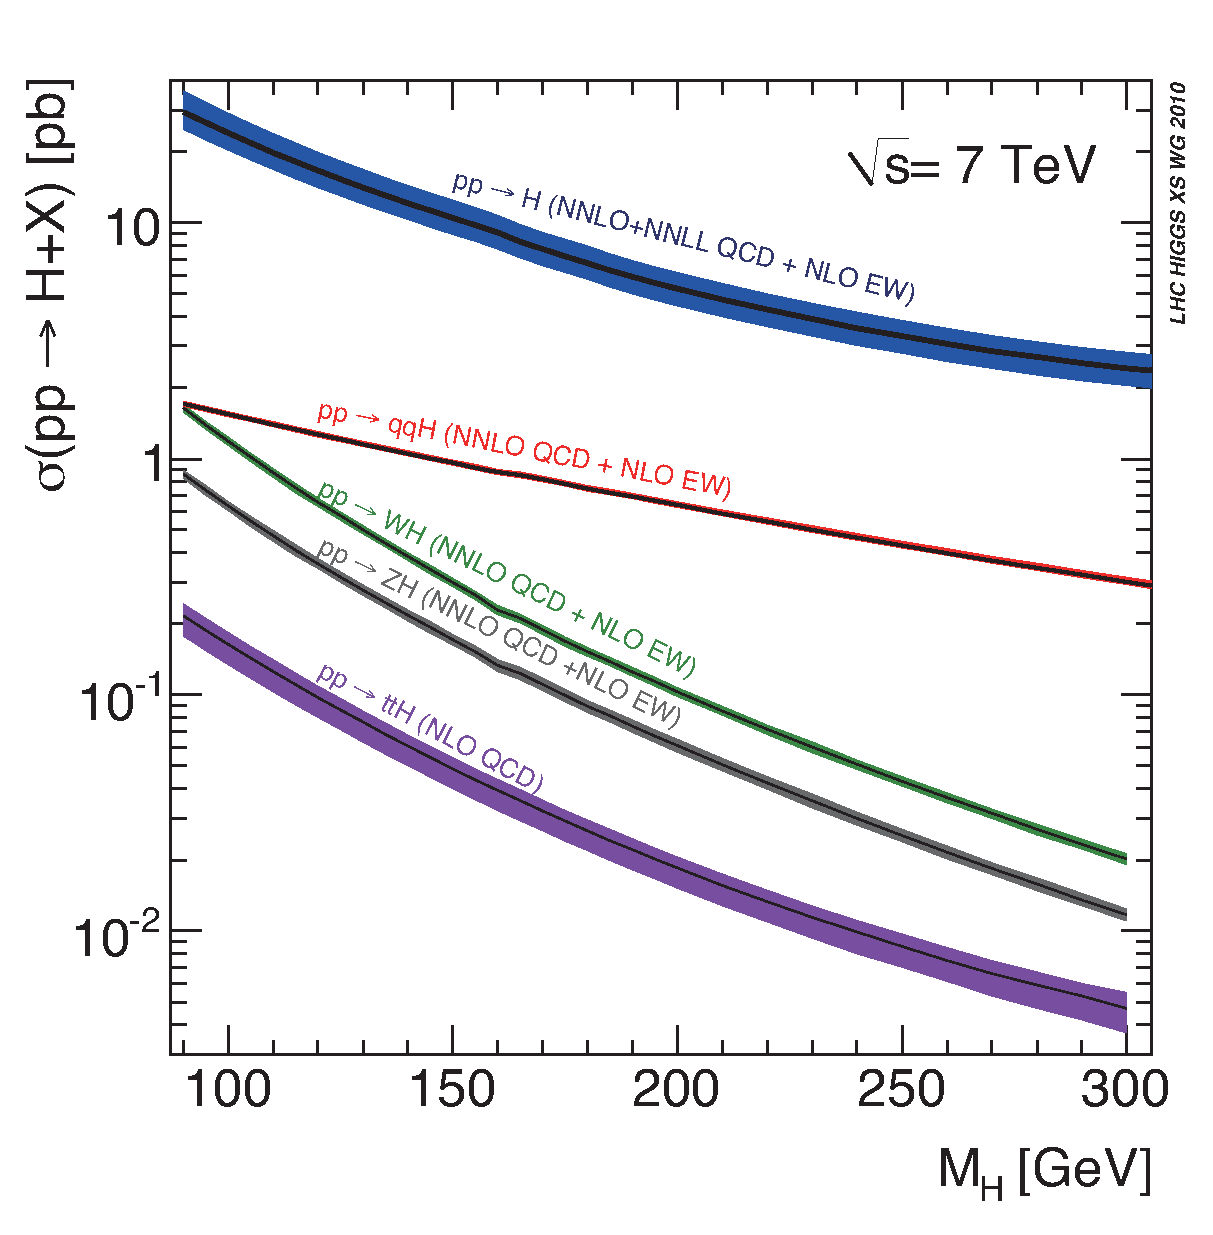
\includegraphics[width=0.48\textwidth]{1_Introduction_Th_and_Exp/pics/Higgs_XS_7TeV_LM.eps}
	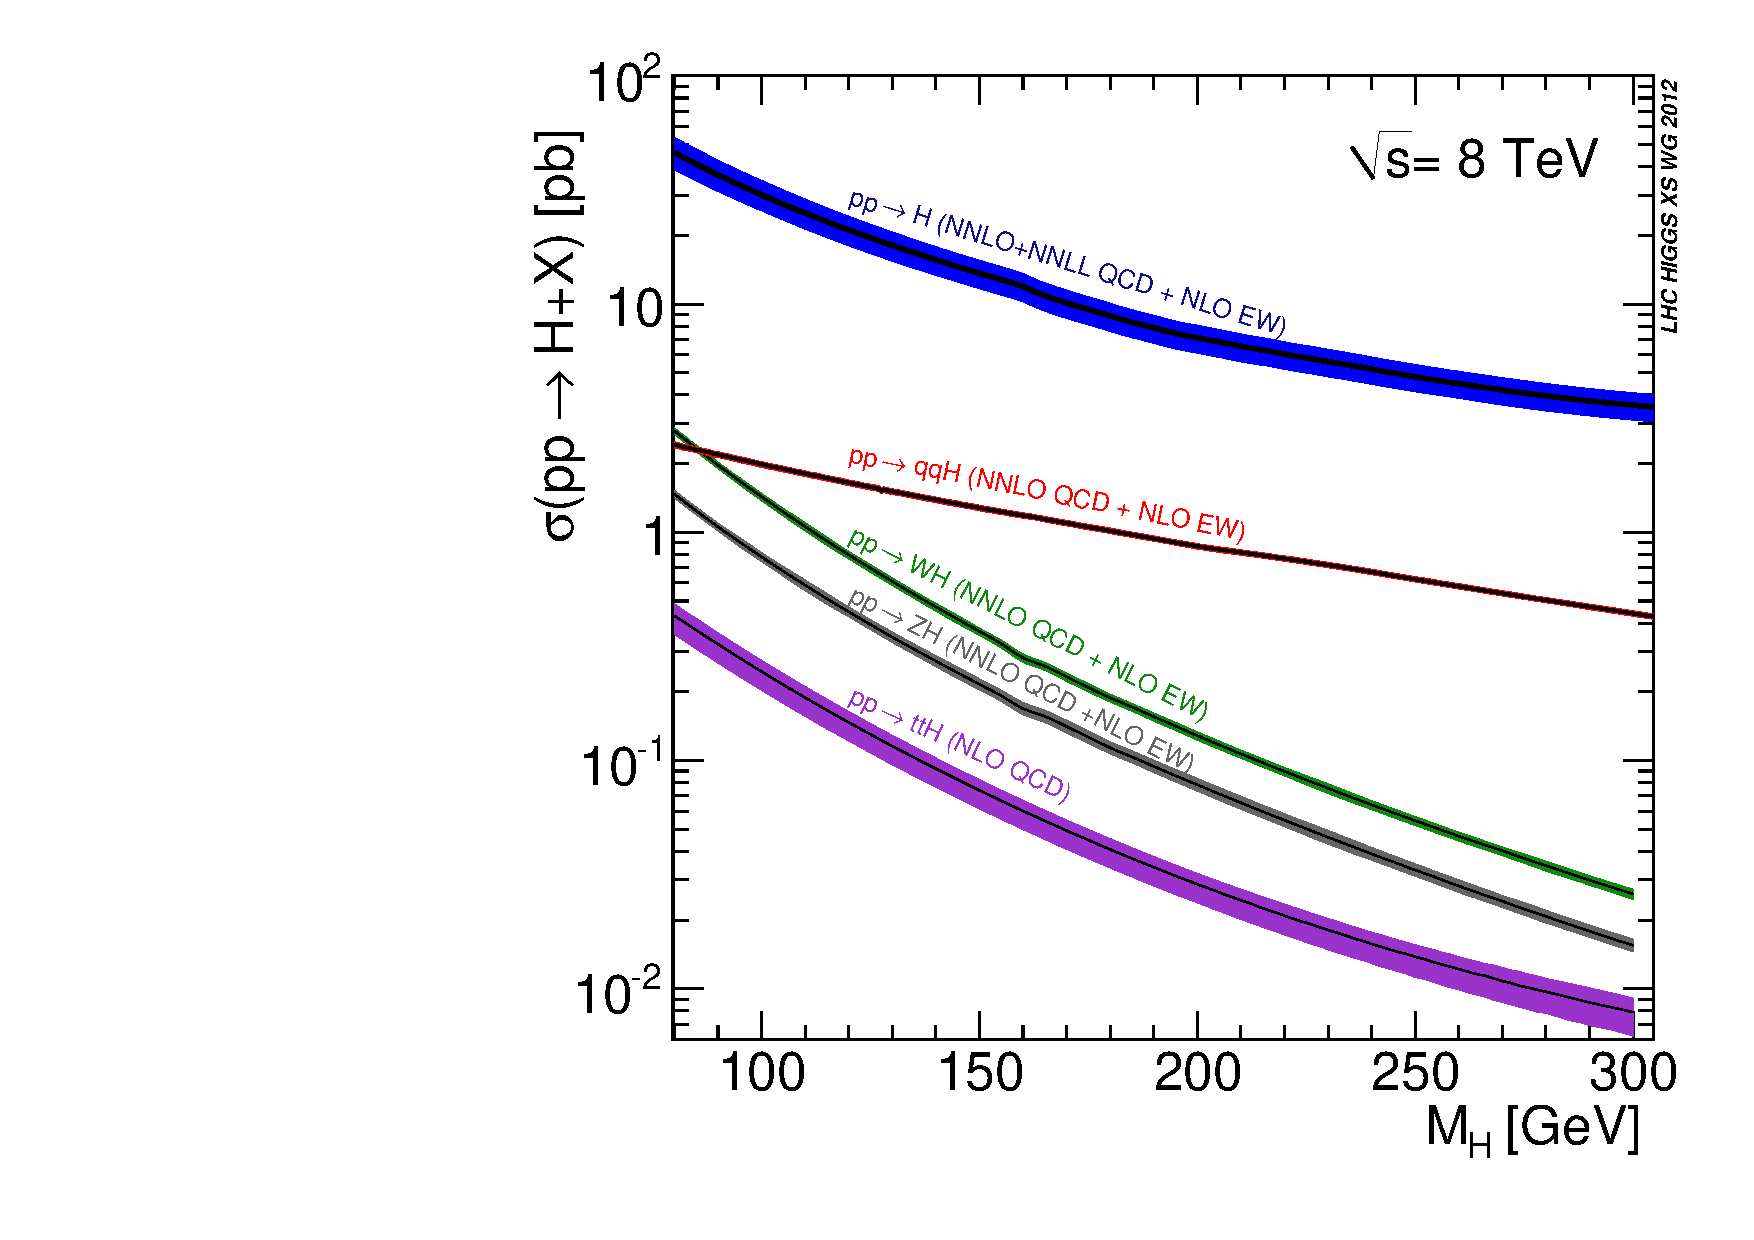
\includegraphics[width=0.48\textwidth]{1_Introduction_Th_and_Exp/pics/Higgs_XS_8TeV_LM.pdf}
       \caption{Higgs production cross section at 7 TeV (left) and 8 TeV (right). The bands represent the theoretical uncertainties on the computation.}
       \label{fig:hxs}
\end{figure}


\subsection{Higgs decays}

Even though the couplings of the Higgs boson are dictated by the mass of the fundamental particles, the branching ratio of the Higgs boson to fundamental particles is dependent on the Higgs mass, as a phase--space factor is added. The running of the main decay modes for the Higgs boson as a function of its mass are shown in Figure \ref{fig:hbr}. 

\begin{figure}
\centering
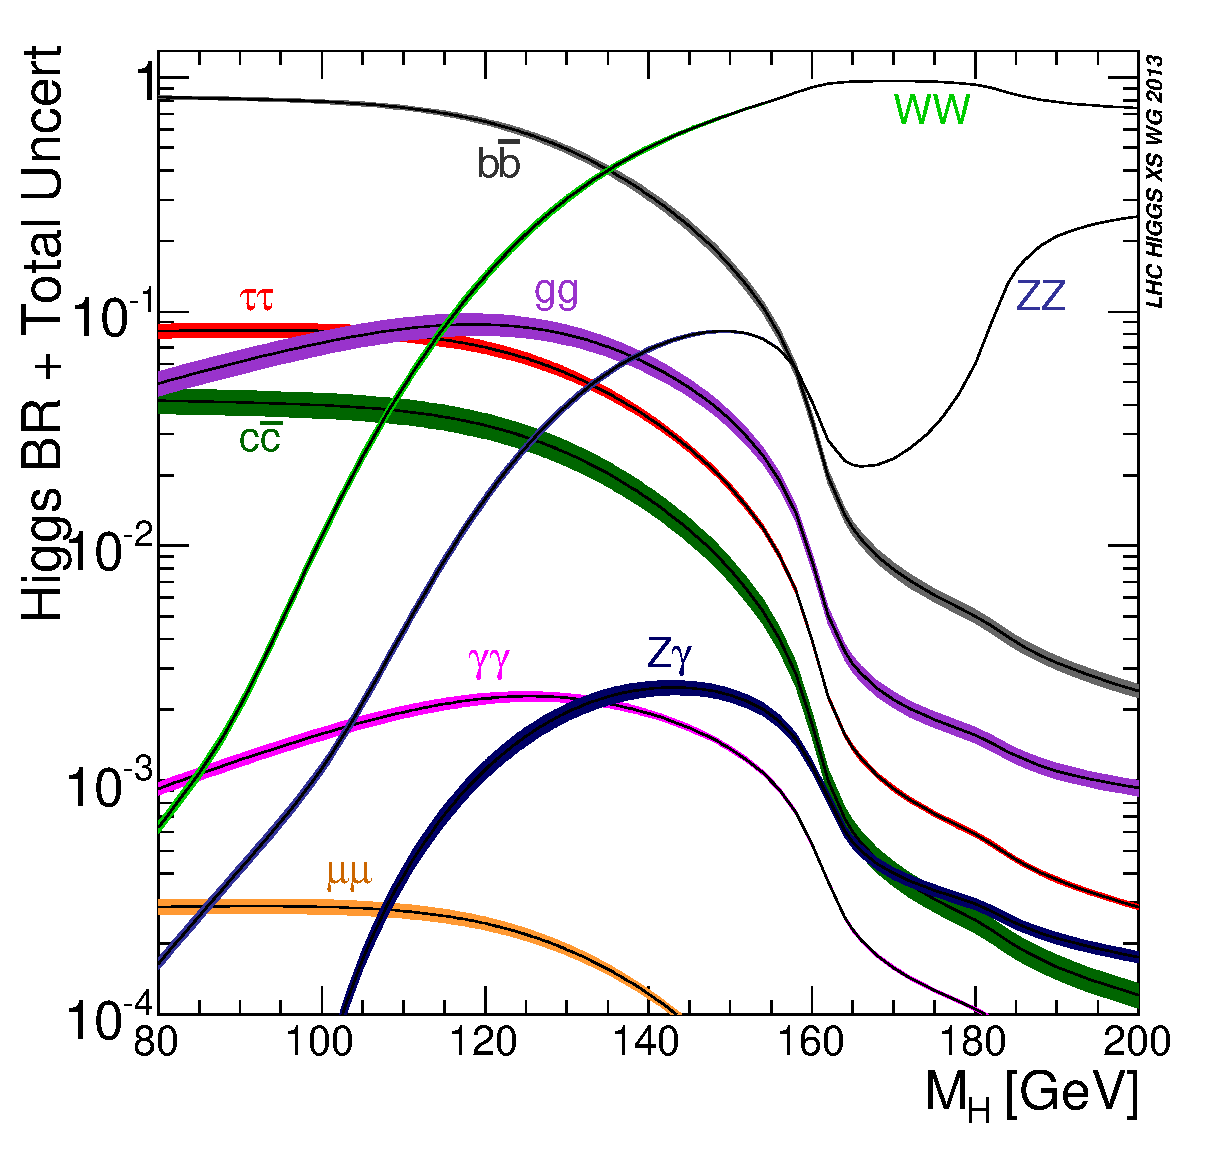
\includegraphics[width=0.5\textwidth]{1_Introduction_Th_and_Exp/pics/Higgs_BR_LM.eps}
\caption{Higgs branching ratios to different fundamental particles as function of Higgs mass.}
\label{fig:hbr}
\end{figure}

From this picture it is possible to notice that even though the Higgs boson has no direct coupling to the photon, a seizable branching ratio is anyway achieved through loop contributions. These loops, as in case of the gluon fusion could contain contributions from new physics making this process a viable channel to probe theories beyond the stand model.

\section{Higgs boson searches}

The first evidence of a new resonance at the mass of 125 GeV compatible with the SM Higgs has been announced by the ATLAS and CMS experiments on the 4$^{th}$ of July 2011 \cite{Chatrchyan:2013lba}. This first evidence has been based on analyses searching for the Higgs boson in decay channels with gauge bosons, mainly ZZ$^*$ and $\gamma\gamma$.

Currently, the significance of the Higgs boson signal exceeds 5$\sigma$ for $\H\To\gamma\gamma$ searches in both CMS and ATLAS \cite{Khachatryan:2014ira, ATLASCONF:2014009}. A similar situation is also present in the ZZ and WW channels.

The high significance of these channels has allowed to perform initial studies on the properties of the resonance. The high invariant mass resolution of $\gamma\gamma$ and ZZ channels has allowed to measure the mass of the boson with high precision: $m_\H = 125.36 \pm 0.37\, \rm{(stat)} \pm 0.18\, \rm{(syst)}$ GeV and $m_\H = 125.03^{+0.26}_{-0.27} \,\rm{(stat)}^{+0.13}_{-0.15}  \,\rm{(syst)} = 125.03^{0.29}_{-0.31} \, \rm{(tot)}$ GeV for ATLAS \cite{Aad:2014aba} and CMS \cite{CMS:2014ega}, respectively.

The spin and parity ($J^P$) of the resonance has also been characterized by dedicated studies on the ZZ and WW channels, which decay topology is more sensitive to these physical observables. The results \cite{CMS:2014gga}, shown in Figure \ref{fig:hjp}, exclude any concurrent hypothesis at more than 99\% confidence level (CL), leaving only $0\+$ as an option.

\begin{figure}
        \centering
	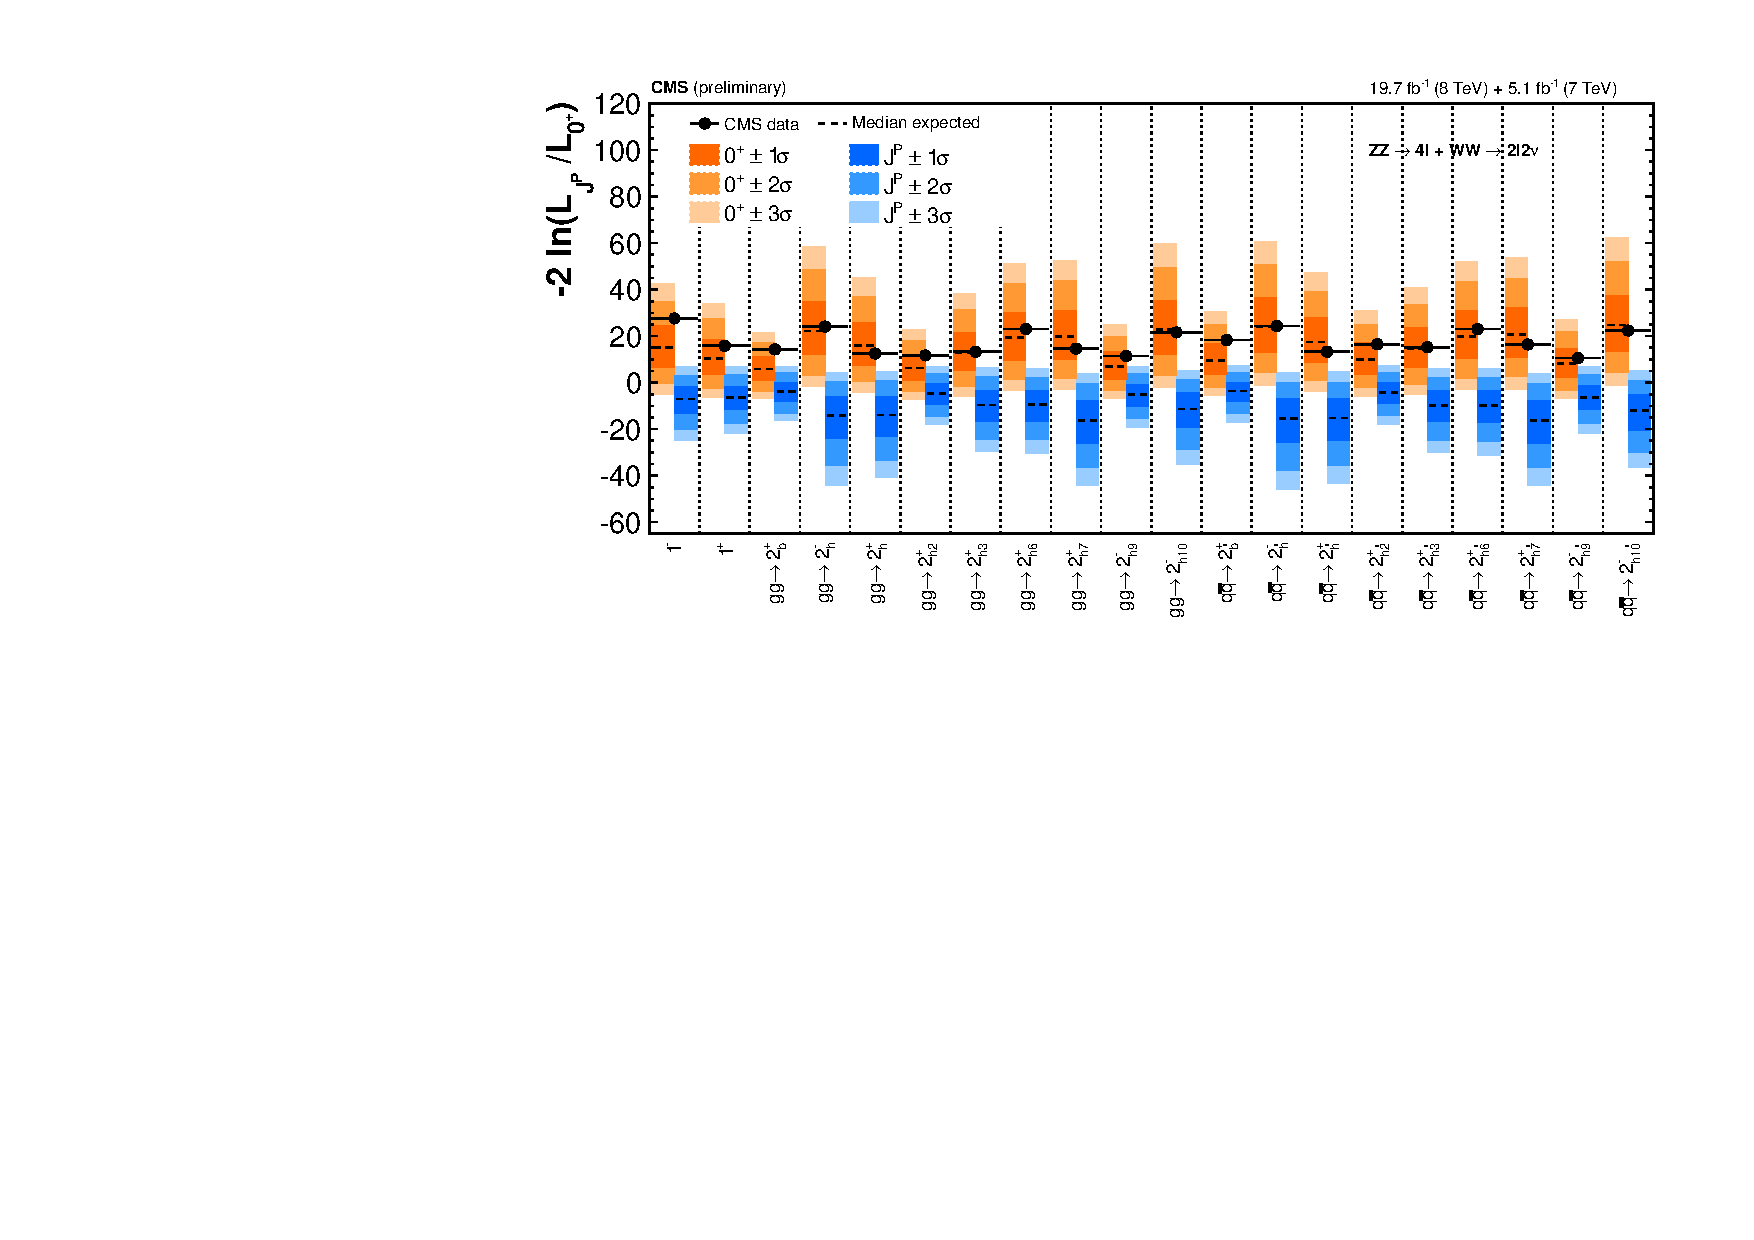
\includegraphics[width=0.8\textwidth]{1_Introduction_Th_and_Exp/pics/hwwhzz_JP_SummaryPlot.pdf}
       \caption{Summary of different $J^P$ hypotheses tested against the $0\+$ one using ZZ and WW Higgs decay data. The orange and blue bands represent the 1?, 2?, and 3? around the median expected value for the SM Higgs boson hypothesis and the alternative hypothesis hypothesis, respectively. The black point represents the observed value. }
       \label{fig:hjp}
\end{figure}

The theoretical SM Higgs boson width for $m_\H \approx 125$ GeV boson is $\Gamma_\H \approx 4$ MeV way below the mass resolution of both detectors. It has been possible, though, to measure with better precision the upper limit of the width from the ratio between on--shell and off--shell event yields, obtaining $\Gamma_{obs} / \Gamma_\H < 5.3$ for CMS \cite{Khachatryan:2014iha} and $\Gamma_{obs} / \Gamma_\H < 5.7$ for ATLAS \cite{ATLASCONF:2014042}. 

The search for Higgs boson decays to bottom quark pairs is the only feasible search of Higgs decays to down--type quarks at hadronic colliders, as the coupling to the other two quarks are largely suppressed by their mass while the hadronic background increases dramatically. The large background contamination in $\H\To b\bar{b}$ restricts the searches to all production processes but the gluon fusion, allowing for the richer final state to be used to remove most of the backgrounds.

Currently no evidence has been found of Higgs decays to $b$--quark pairs, but CMS reported a $2.1\sigma$ excess in the VH production \cite{Chatrchyan:2013zna}, compatible with the SM predictions. The equivalent analysis for ATLAS does not show any excess \cite{TheATLAScollaboration:2013lia}, but is also less sensitive.

The branching fraction of the Higgs boson to muon pairs is predicted to be very low, therefore any excess might be a strong indication of new physics. Both ATLAS \cite{Aad:2014xva} and CMS \cite{CMS:2013aga} performed a search for such decay, exploiting the extremely good resolution that can be achieved in this channel, without finding any significant excess so far. The analyses set an independent upper limit on the branching ratio approximately 7 times the SM expectation.

The only direct observation of SM Higgs coupling to top quarks can be observed in the $tt$H associated production, since the low mass of the Higgs boson forbids such decay. The search for $tt$H is performed in many Higgs final states. Both ATLAS and CMS exploit the $b\bar{b}$ and $\gamma\gamma$ final states; additionally CMS searches for this production mode also in multi-lepton final states, targeting the $\tau\tau$ and WW Higgs decay modes.

The combination of these searches leads in CMS to a $3.5\sigma$ excess with respect to the background--only hypothesis \cite{CMS:2014ega}. The combined \emph{signal stranght} ($\mu$), i.e. the ratio $\mu = (\sigma \times BR)_{obs} / (\sigma \times BR)_{SM}$, is $\mu = 2.76^{+1.05}_{0.92}$ which is two standard deviations away from the SM expectation ($\mu = 1$). The excess in this combination is driven by the same--sign dimuon analysis, which looks for $\H\To \W\W$, and $\H\To\gamma\gamma$. The results from ATLAS show a mild, non conclusive, excess \cite{ATLASCONF:2014043}.

The $\H \to \tau \tau$ decay mode is searched for in gluon fusion, VBF (CMS and ATLAS) and associated production (CMS only). In CMS \cite{H_tautau}, events are selected on--line by dedicated triggers and selected according the isolation of the final state leptons. Events are separated into categories tailored around specific production mechanisms (VBF, VH, gluon fusion) and, in the gluon fusion case, according to the boost of the hadronic tau and Higgs candidate. The invariant mass spectrum of the Higgs final states is smeared in this decay mode due to the presence of neutrinos in the tau lepton decay. To recover this effect, a dedicated likelihood integration method, called SVFit, performs the di-tau invariant mass calculation taking as input the momenta of the visible Higgs products and the missing transverse energy (\MET) information. The resolution achieved with this technique, that can be applied only where the taus are the only source of missing energy, varies between 10 and 20\%, depending on the final state and the category.

Most of the backgrounds present in the direct production (VBF and gluon fusion) categories are modeled using simulated events with dedicated sideband regions to cross--check the simulation and apply correction factors where needed. The main background for these categories is given by $\Z \To \tau\tau$ events which are modeled with \emph{embedded Monte Carlo} techniques: real $\Z \To \mu \mu$ events are selected from collision data and the two muons are replaced with simulated tau decays, after correcting for the appropriate phase space factor.

A combined fit to all the channels and categories reveals a $3.2\sigma$ deviation from the background--only hypothesis and a combined $\mu = 0.78 \pm 0.27$, well compatible between channels as shown in Figure \ref{fig:htt_mu}. The best-fit mass, $m_\H = 122 \pm 7$ GeV, is also compatible with the ZZ and $\gamma\gamma$ value. Similar results are obtained by ATLAS \cite{ATLASCONF:2013108}, with a $4.1\sigma$ deviation from the background--only hypothesis and $\mu = 1.4^{+0.5}_{-0.4}$, slightly in excess, but still compatible, with respect to the SM value.

\begin{figure}
        \centering
	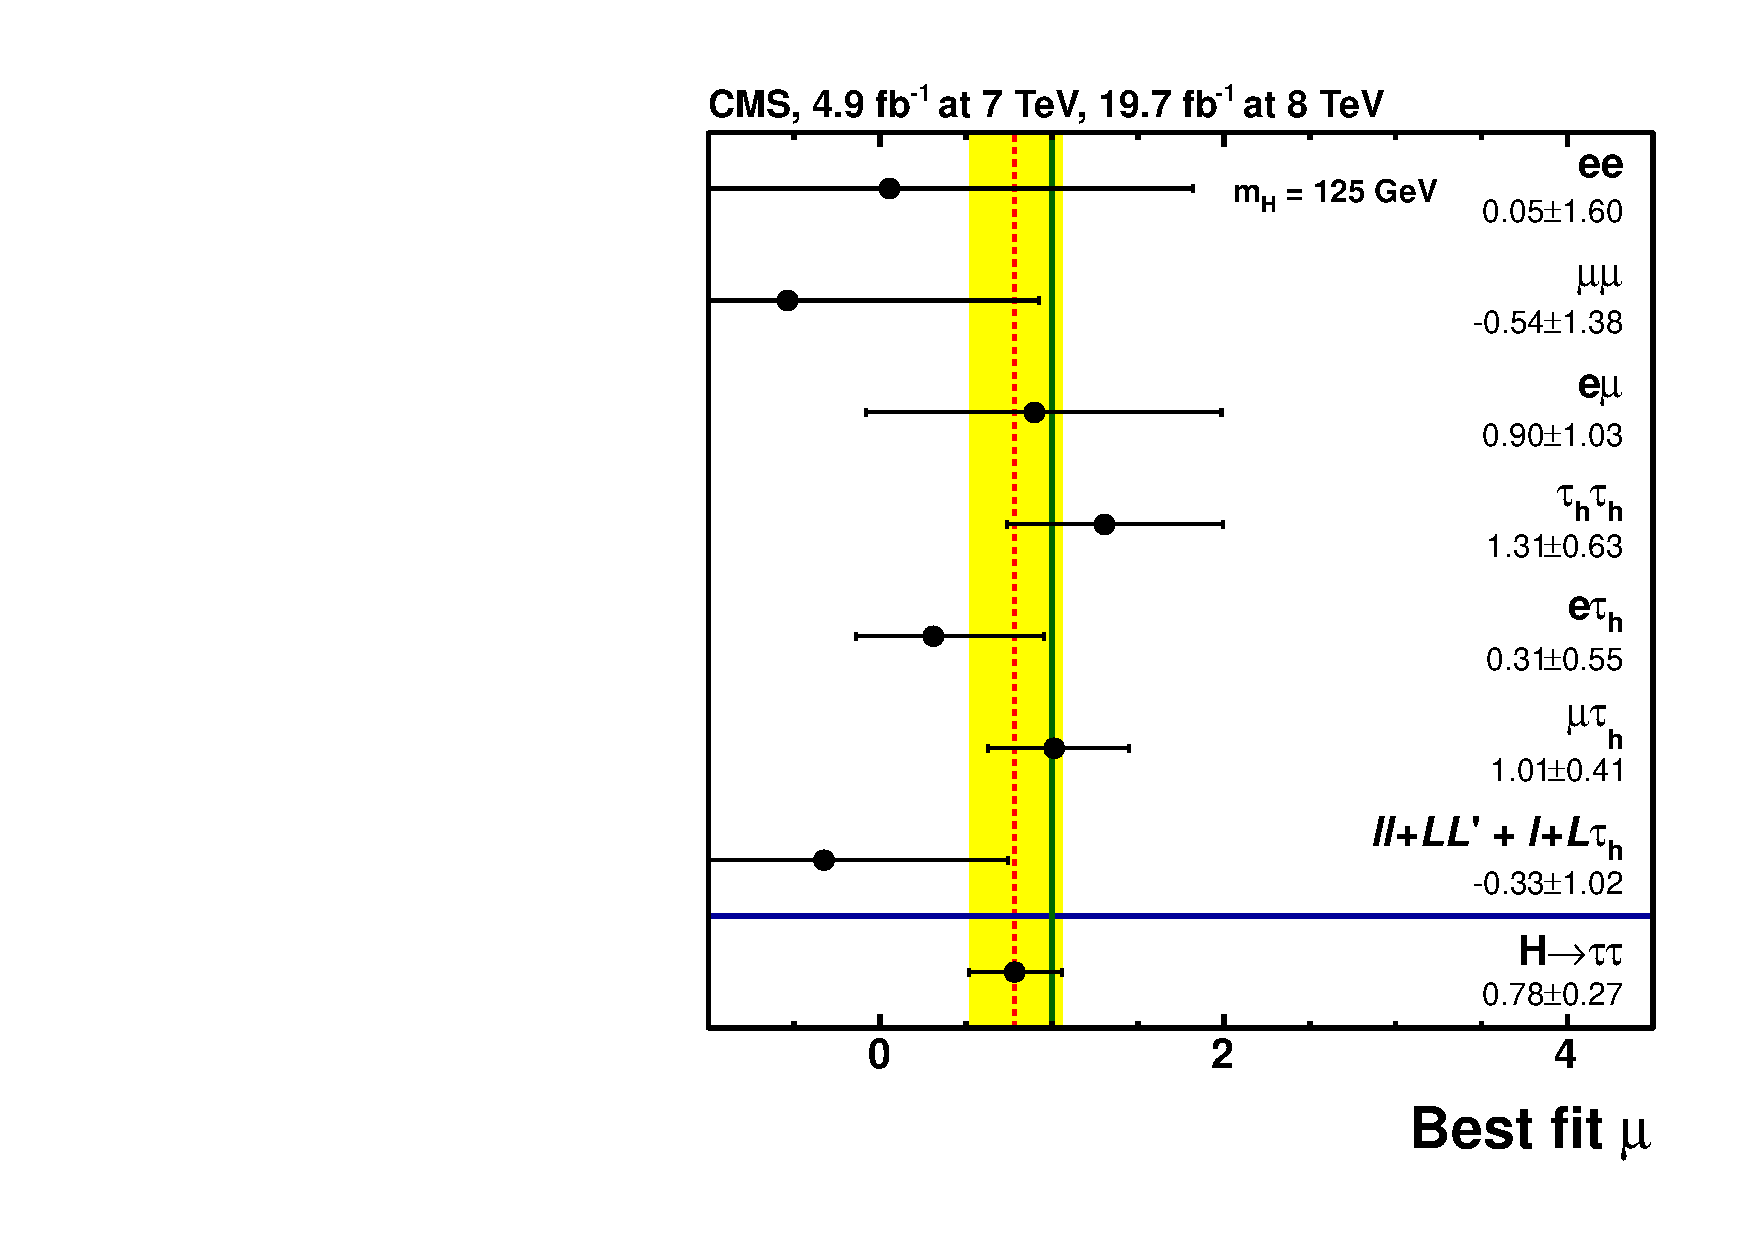
\includegraphics[width=0.6\textwidth]{1_Introduction_Th_and_Exp/pics/BestFit_sm_per_chn.pdf}
       \caption{ }
       \label{fig:htt_mu}
\end{figure}

The $\H \To b\bar{b}$ and $\H \To \tau \tau$ results can be combined leading to a $3.8\sigma$ combined evidence of Higgs coupling to down--type fermions from CMS \cite{Chatrchyan:2014vua}.

The outcome of the various searches have been combined by the single experiments in a simultaneous fit to better determine the couplings of the Higgs boson to the different fundamental particles. The result of the single and combined signal strengths for both ATLAS \cite{ATLASCONF:2014009} and CMS \cite{CMS:2014ega} is presented in Figure \ref{fig:combination}.

\begin{figure}
        \centering
	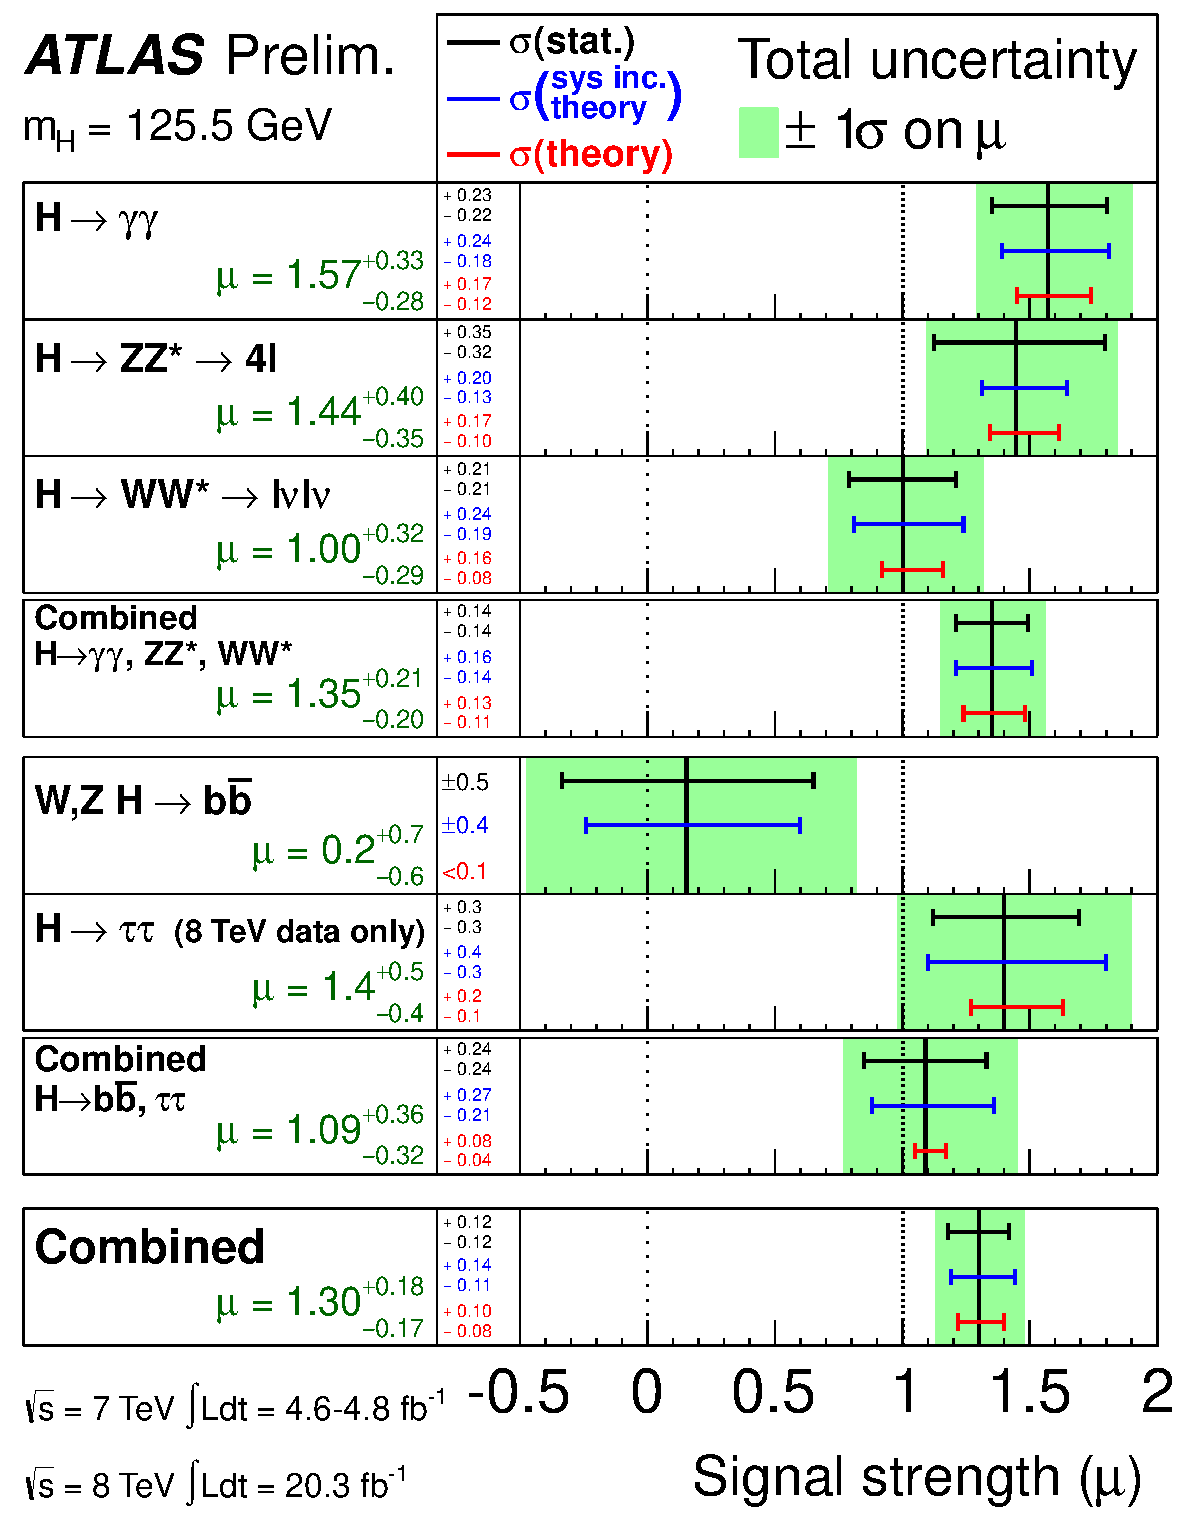
\includegraphics[width=0.39\textwidth]{1_Introduction_Th_and_Exp/pics/fig_01.pdf}
	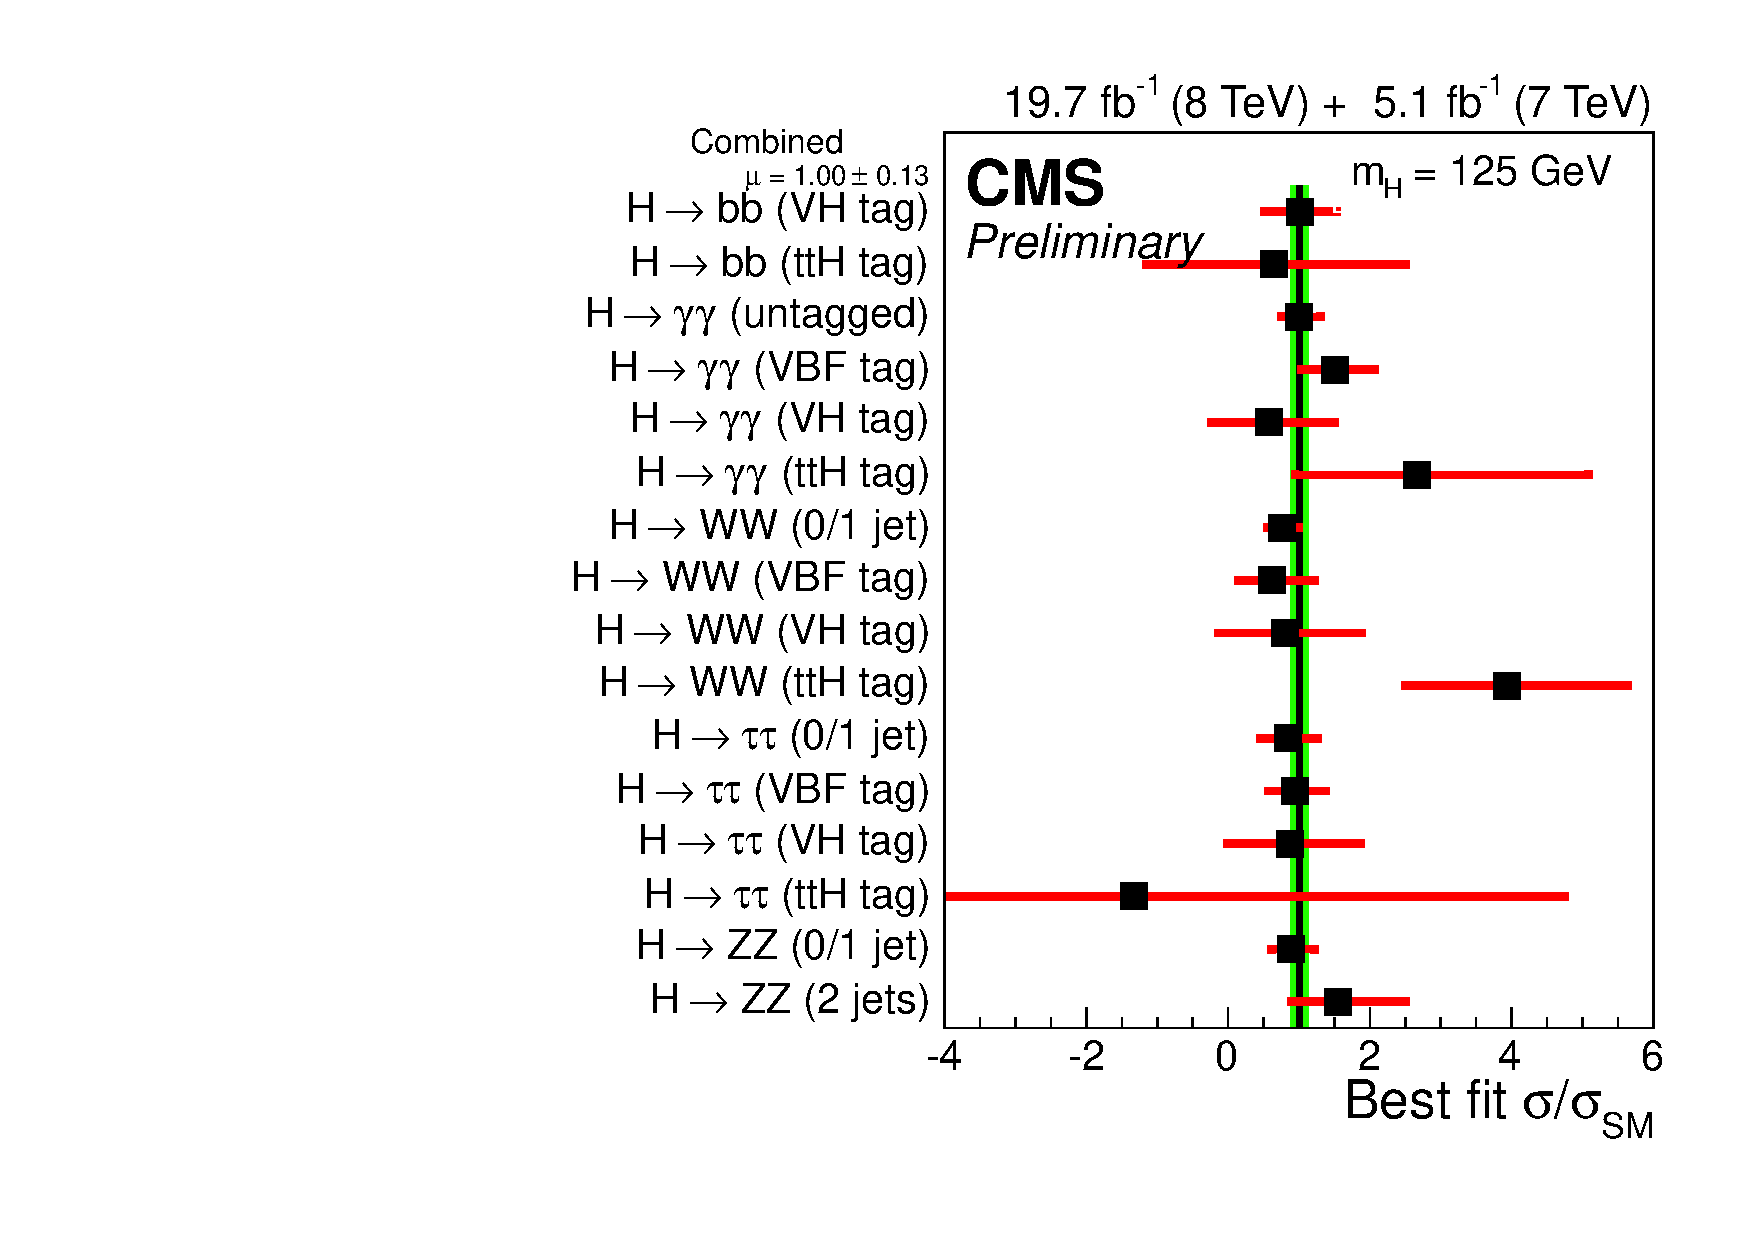
\includegraphics[width=0.54\textwidth]{1_Introduction_Th_and_Exp/pics/sqr_mlz_ccc_mH125.pdf}
       \caption{ }
       \label{fig:combination}
\end{figure}

Another way to interpret the results is to compute the couplings of the Higgs boson to gauge bosons ($k_V$) and to fermions ($k_F$) and to plot the one--sigma contour regions allowed by each measurement. This interpretation assumes the absence of new physics in loop processes to infer information of the different production processes (e.g. assumes that the gluon fusion is almost completely mediated by a top loop). This interpretation of the results is available in Figure \ref{fig:kvf} for both the experiments.

\begin{figure}
        \centering
	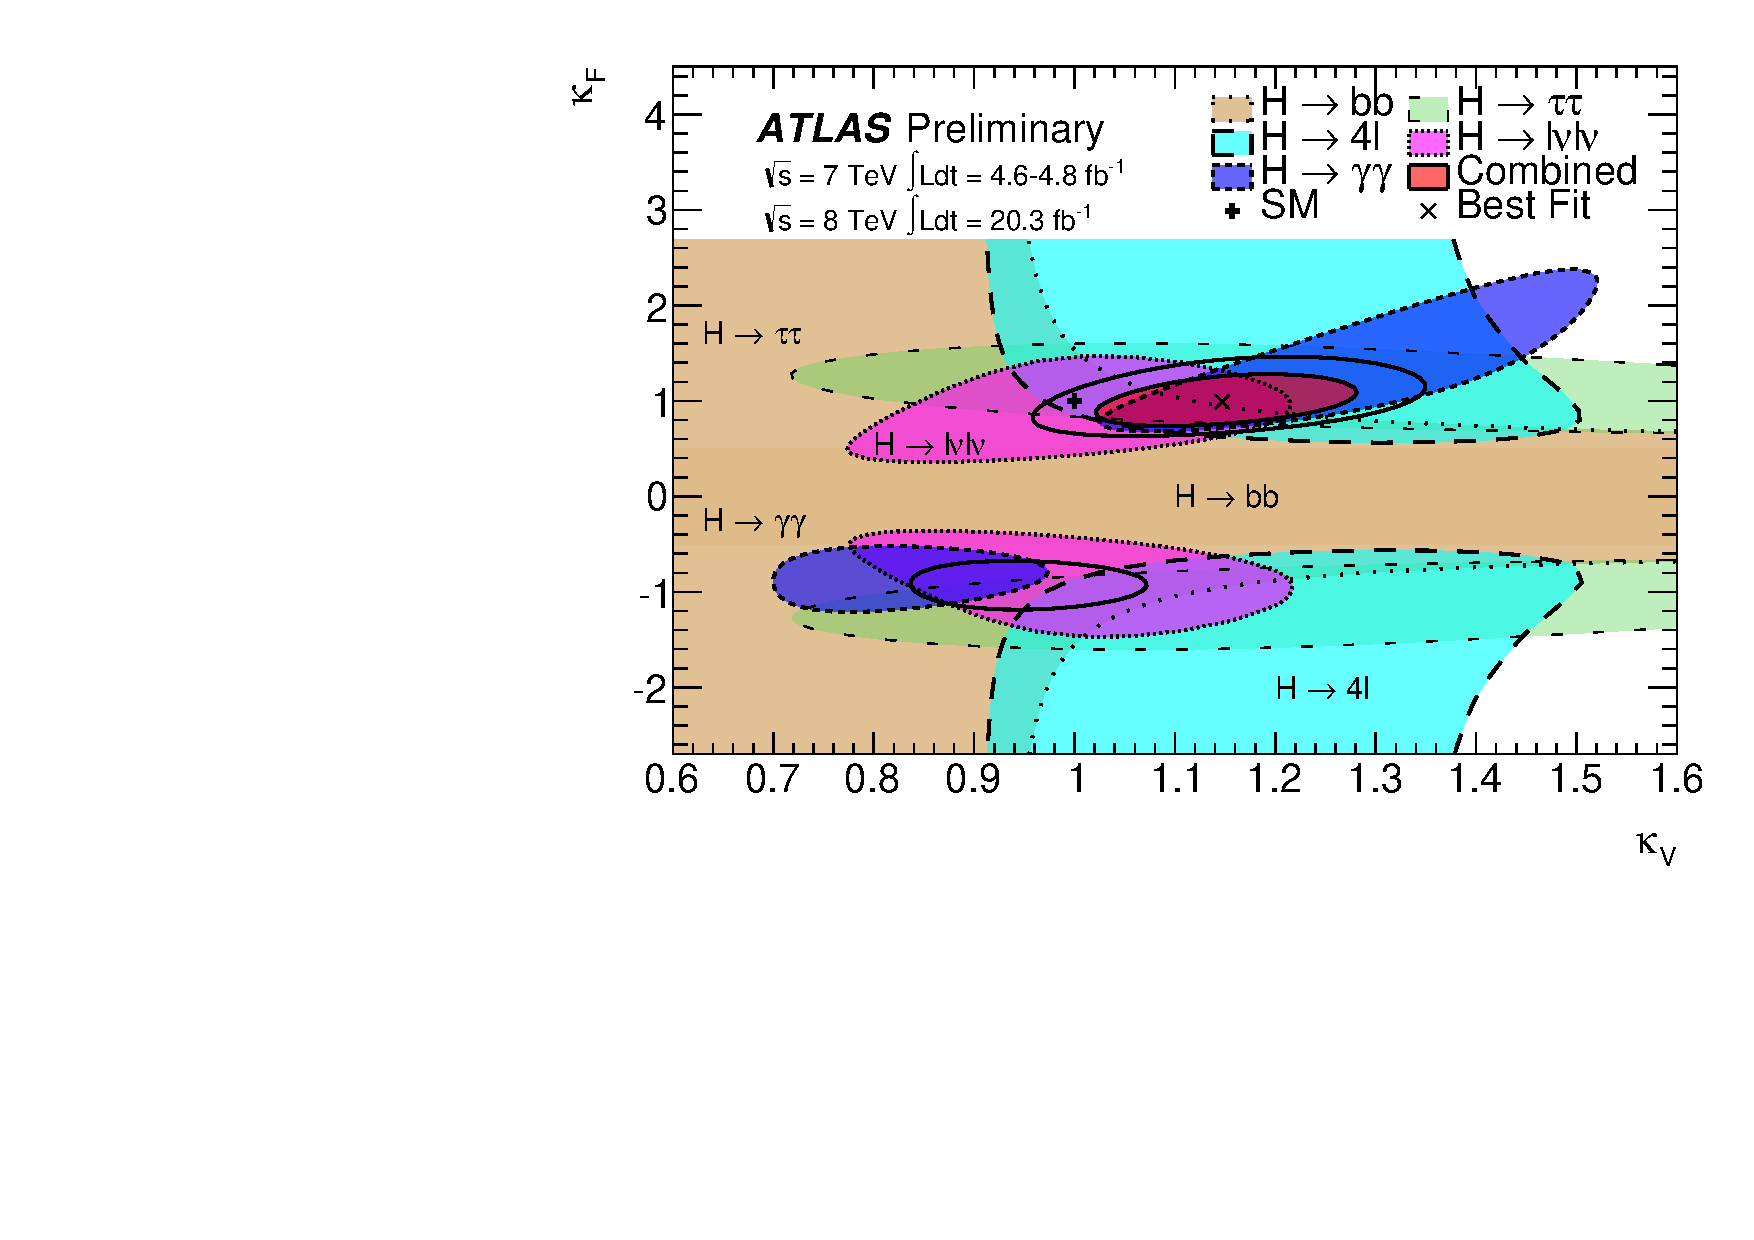
\includegraphics[width=0.53\textwidth]{1_Introduction_Th_and_Exp/pics/fig_05b.pdf}
	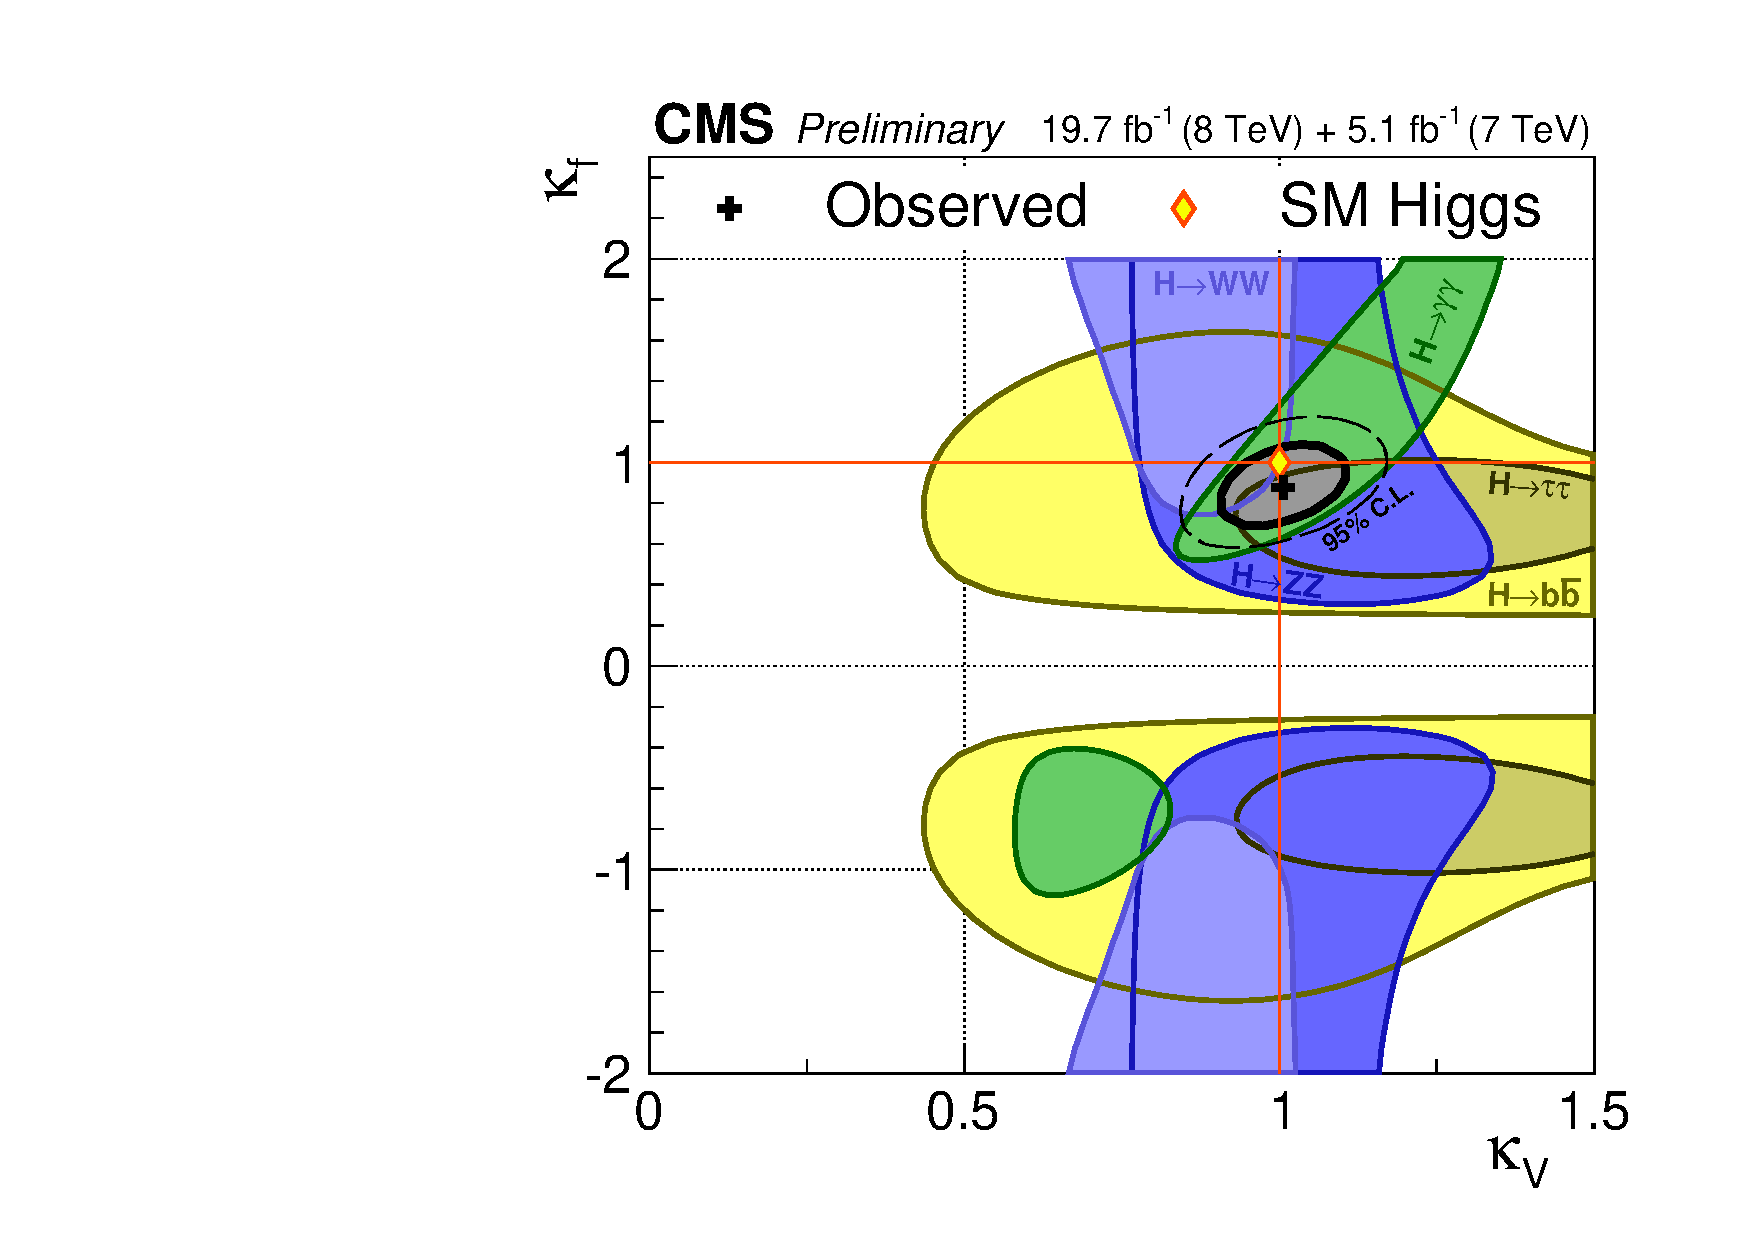
\includegraphics[width=0.41\textwidth]{1_Introduction_Th_and_Exp/pics/cVcF_all_channels_2quadrant.pdf}
       \caption{ }
       \label{fig:kvf}
\end{figure}

All the results found so far by both ATLAS and CMS experiments are compatible with the interpretation of this new resonance as a purely SM Higgs boson, but the precision of such measurements still allows plenty of room for new physics processes.

%In the following part of this work a more detailed description of the $\W\H \To \ell \ell \tau$ analysis will be shown. This 


